%Plantilla Memoria Técnica:
%Modificada por: Brenda Mariana Casillas González
%Última Modificación: 02-01-2023

%------------------------------CONFIGURACION DEL DOCUMENTO

\documentclass[12pt,letterpaper,spanish]{report}
\usepackage[table]{xcolor} 
\usepackage[centertags]{amsmath}
\usepackage{amsfonts}
\usepackage{amssymb}
\usepackage{amsthm}
\usepackage[T1]{fontenc}
\usepackage[utf8]{inputenc}
\usepackage{lmodern}
\usepackage[spanish,activeacute]{babel}
% Eliminar o comentar cualquier redefinición de fuentes para evitar conflictos
% \renewcommand{\rmdefault}{lmr}
% \renewcommand{\sfdefault}{lmss}
% \renewcommand{\ttdefault}{lmtt}
\usepackage{epsfig}
\usepackage{booktabs}
\usepackage{graphicx}
\renewcommand{\baselinestretch}{1.5}
%\usepackage[numbers]{natbib}
\usepackage[round]{natbib}
\usepackage[hyphens]{url}
\usepackage{enumerate}
\usepackage{hyperref}
\usepackage{array}
\usepackage{float}

\newenvironment{dedication}{\newpage\large\null\em\vskip1in}%
{\vfill}

\topmargin -1 in \oddsidemargin 0in \evensidemargin 0in
\textwidth 6.5in
\textheight 9in \pagestyle{myheadings}

% -----------------------------------INICIO DEL DOCUMENTO  ---------------------------------------------------------------
\begin{document}


% Para la elaboración de esta memoria técnica se debe usar un editor profesional que soporte Latex, como recomendación se puede usar el WinEdt.

% El resultado que se sube a la plataforma debe ser en formato PDF

% Es importante mencionar que la redacción de este documento se debe hacer en tercera persona, cuidando escrupulosamente la ortografía, redacción y contenido, evitando el uso y abuso de adjetivos.

    
% ----------------------------------- CONTRAPORTADA -------------------------------------------------------------------------
%Se deben modificar los datos de la empresa, proyecto, asesores y alumnos




% ------------------------------  PORTADA -----------------------------------------------------
%Se deben modificar los datos de la empresa, proyecto y alumnos


\thispagestyle{empty}


\begin{center}

 \begin{minipage}[b]{.9\linewidth}
    \begin{center}
        \vspace{0.2in}
        \large{UNIVERSIDAD TECNOLÓGICA DE LA ZONA \\METROPOLITANA DE GUADALAJARA}\\
        \large{DIRECCIÓN DE DESARROLLO Y GESTIÓN DE SOFTWARE}\\
    \end{center}
\end{minipage}
\vspace{0.3in}


\centerline{\hbox{\psfig{file=logoUTZMG.jpg,height=2in,width=1.5in}}}

\LARGE{\textsc{Sistema de Gestión de Reprocesos y Pedidos}}
% \LARGE{\textbf{Módulo de Gestión de Reprocesos y Reposiciones}} % Alternative: bold only, no small caps

\vspace{0.2in}
\large{\textbf{MEMORIA TÉCNICA REALIZADA EN:}}
 \\  \textsc{Corporativo Textil JSN, S. de R.L de C.V}

\vspace{0.2in}
\large{\textbf{PARA OBTENER EL GRADO DE:}}

\large{Técnico Superior Universitario (TSU) en:}


\large{TECNOLOGÍAS DE LA INFORMACIÓN\\Área, DESARROLLO DE SOFTWARE MULTIPLATAFORMA }
\\

\vspace{0.2in}
\large{PRESENTADO POR:}


\textsc{Víctor Manuel Montaño Juanpedro}  %(Empezando con el nombre  y después apellidos)


\textsc{Eduardo Isaías Vázquez Solís}  %(Empezando con el nombre  y después apellidos)

\vspace{0.2in}
\small{ AGOSTO 2025}
\end{center}
%\vspace{0.1in}


\newpage

\thispagestyle{empty}

\begin{table}[ht]
  \centering
    \begin{tabular}{rr}
        \begin{minipage}[b]{0.05\linewidth}
        \hbox{\psfig{file=LogoUTZMG.jpg,height=1in,width=.8in}}
        \end{minipage}
    &
    \begin{minipage}[b]{.8\linewidth}
        \begin{center}
            \large{UNIVERSIDAD TECNOLÓGICA \\ DE LA ZONA METROPOLITANA DE GUADALAJARA}\\
        \end{center}
    \end{minipage}

    \end{tabular}%
\end{table}%

\begin{center}

\large{\textbf{MEMORIA TÉCNICA REALIZADA EN:}}
 \\  Corporativo Textil JSN, S. de R.L de C.V

%%Logo de la empresa
\centerline{\hbox{\psfig{file=LogoJASANA.png,height=0.4in,width=1.2in}}}

\large{\textbf{PROYECTO:} Sistema de Gestión de Reprocesos y Pedidos}

\vspace{0.1in}
\large{\textbf{PARA OBTENER EL GRADO DE:}}

\large{Técnico Superior Universitario (TSU) en:}
\vspace{0.05in}

\large{TECNOLOGÍAS DE LA INFORMACIÓN, ÁREA DESARROLLO DE SOFTWARE MULTIPLATAFORMA }
\\
\large{PRESENTADO POR:}


Víctor Manuel Montaño Juanpedro %(Empezando con el nombre  y después apellidos)


Eduardo Isa'ias V'azquez Solís %(Empezando con el nombre  y después apellidos)

\vspace{0.5in}

\begin{tabular}{cc}
    %\vspace{0.5in}
    \textbf{ASESOR INDUSTRIAL} & \textbf{ASESOR ACADÉMICO} \\

    Jair Efra'in Barragán Gárcia & Lizbeth Noriega Gútierrez \\
    \multicolumn{2}{c}{\textbf{COORDINADOR DE CARRERA}
    \vspace{0.4in}
    } \\

    \multicolumn{2}{c}{
            Mtra. Lizbeth Noriega Gútierrez }
    \end{tabular}

\end{center}
%\vspace{0.1in}
\begin{flushright}\small{ TLAJOMULCO DE ZÚÑIGA, JALISCO, AGOSTO DEL 2025} \end{flushright}



% -------------------------------------- DEDICATORIA   ---------------------
% Esta sección es opcional, pero se recomienda que se ponga, se puede redactar hasta el final y tratar que no sea mayor a una cuartilla.

        \thispagestyle{empty}
        \addcontentsline{toc}{chapter}{Agradecimientos}

\begin{dedication}
  \textbf{Agradecimientos Víctor Manuel Montaño Juanpedro}


En primer lugar, expreso mi sincero agradecimiento a la \textbf{Maestra Lizbeth Noriega Gutiérrez}, mi asesora académica, por su guía, paciencia y compromiso durante la elaboración de esta tesis. Su acompañamiento fue clave para alcanzar los objetivos propuestos.

Extiendo mi agradecimiento al \textbf{Lic. Jair Efraín Barragán García}, asesor industrial de este proyecto, por compartirnos su experiencia en los procesos operativos de la empresa. Su apoyo fue fundamental para entender el entorno real donde se implementaría esta solución.

A la \textbf{Ingeniera María de Jesús García Herrera}, directora general de \textit{Corporativo Textil JSN}, gracias por brindarme la oportunidad de realizar mis estadías profesionales en la empresa, por su confianza a lo largo del proceso.

A mis padres, \textbf{Juan Manuel Montaño Guevara} y \textbf{Yolanda Juanpedro Don}, les agradezco profundamente por esfuerzo y por haberme brindado siempre los medios y el respaldo necesarios para seguir adelante con mis estudios. Este logro es tan mío como suyo.

Por último pero no menos importante, a mi novia, \textbf{Claudia Lorena Espinoza Rubalcava}, gracias por tu apoyo incondicional y tu compañía constante. Tu presencia en cada paso de este camino fue una fuente de ánimo y motivación.

\end{dedication}
    

\newpage
\begin{dedication}
    \textbf{Agradecimientos Eduardo Isaías Vázquez Solís}
 
 
 
  Quiero comenzar expresando mi más sincero agradecimiento a la \textbf{Universidad Tecnológica de la ZMG (UTZMG)} por brindarme los conocimientos y herramientas necesarias para afrontar los retos del mercado laboral. Su formación ha sido fundamental en mi crecimiento profesional y personal.

    A la \textbf{Maestra Lizbeth Noriega Gutiérrez}, por su valiosa labor como asesora y consejera, no solo durante este periodo de estadías, sino también por su constante acompañamiento desde los inicios de mi carrera. Su guía, paciencia y apoyo han sido imprescindibles para el desarrollo de este proyecto.
    
    A mis compañeros de grado y amigos, quienes con su apoyo, comprensión y compañerismo han hecho este proceso mucho más llevadero y agradable. Gracias por compartir este camino y por las experiencias vividas juntos.

    Mi más profundo agradecimiento a mi madre, \textbf{Griselda Isabel Solís Gómez}, quien siempre me ha brindado su amor, apoyo incondicional y aliento. A mi padre, \textbf{Domingo Vázquez Hernández}, quien, a pesar de no encontrarse físicamente entre nosotros, me enseñó el valor de la perseverancia y el esfuerzo. Estoy profundamente agradecido por las herramientas que me dio para nunca desistir, siempre creyendo en mi y en mi formación académica.
    \newpage
    A la empresa \textbf{Corporativo Textil JSN}, y en especial a la \textbf{Ingeniera María de Jesús García Herrera}, por brindarme el espacio y la oportunidad de realizar este proyecto en un entorno profesional tan enriquecedor. Gracias por confiar en mí para llevar a cabo este trabajo.

    Finalmente, quiero agradecer al \textbf{Lic. Jair Efraín Barragán García}, por su valiosa guía en el proceso industrial y entendimiento del flujo operativo que nos llevó a la finalización de este proyecto, y a mi compañero \textbf{Víctor Manuel Montaño Juanpedro}, con quien tuve el privilegio de trabajar en equipo. Su dedicación y colaboración fueron esenciales para la realización exitosa de este proyecto.
\end{dedication}

%--------------------------------         ÍNDICE


\tableofcontents


% --------------------------------------- CAPÍTULOS DEL DOCUMENTO  ----------------------------------------
% ____________________________________________________________________________________

\pagenumbering{arabic}
\oddsidemargin 0.2in \textwidth 6.5in \topmargin -0.25in
\textheight 9in \pagestyle{myheadings}

\newpage

% CAPITULO INTRODUCCIÓN. Enmarca y situa el trabajo a realizar. Tiene por objeto proporcionar una visión general del documento.
%____________________________________________________________________________________________________________________


\chapter{Introducción}
\newpage


En un entorno empresarial cada vez más competitivo, la optimización de procesos productivos y administrativos se ha convertido en una prioridad para las organizaciones que buscan mantenerse vigentes y aumentar su eficiencia operativa. Particularmente en el sector textil, donde la calidad del producto y la trazabilidad de los procesos son factores clave, contar con herramientas tecnológicas adecuadas puede marcar una diferencia sustancial en los resultados.

Corporativo Textil JSN, empresa dedicada a la confección de uniformes corporativos, enfrenta actualmente diversos retos relacionados con la gestión de reprocesos y reposiciones de piezas defectuosas durante su línea de producción. A pesar de contar con un sistema ERP como Odoo para la gestión general de la empresa, el proceso de reprocesos no está debidamente integrado ni digitalizado, lo que genera una pérdida de información, falta de trazabilidad, trabajo manual excesivo y dificultades para calcular los costos asociados a las correcciones.

Ante este panorama, surge la necesidad de desarrollar una solución digital especializada que permita controlar, documentar y dar seguimiento a las solicitudes de reproceso, de forma estructurada y eficiente. Este proyecto tiene como objetivo diseñar e implementar un sistema web independiente que funcione de manera complementaria al ERP existente, permitiendo así una mayor flexibilidad en el desarrollo y una interfaz de usuario enfocada en las necesidades específicas de esta operación.

Este documento presenta de forma detallada las etapas del desarrollo del proyecto, desde la identificación de la problemática hasta la implementación técnica del sistema, incluyendo el análisis de requerimientos, el diseño de la solución, la elección del stack tecnológico, así como las pruebas de validación realizadas. También se exponen los objetivos generales y específicos del sistema, los beneficios obtenidos a nivel operativo y las perspectivas de mejora continua a partir de su implementación.

En conjunto, el desarrollo de este sistema representa un paso significativo hacia la transformación digital de los procesos internos de Corporativo Textil JSN, permitiendo a la empresa contar con una herramienta eficiente, moderna y alineada con sus objetivos estratégicos de calidad y control operativo.





% CAPITULO ANTECEDENTES Y DESCIPCIÓN DE LA EMPRESA. Tiene por objeto proporcionar una visión general del documento.
%____________________________________________________________________________________________________________________

\chapter{Antecedentes y Descripción de la Empresa}
\newpage



%Nota: Los puntos que siguen son una propuesta, pongan solo los puntos que apliquen en su empresa y que los permitan poner, también puede agregar otros puntos si lo cree conveniente.

\section{Ubicación}
La empresa Corporativo Textil JSN, S. de R.L de C.V se encuentra ubicada en C. Flaviano Ramos Sur 37, Centro, 45640 Tlajomulco de Zúñiga, Jal. El mapa puede ser consultado en la Figura\ref{a01}

\begin{figure}[htp]
  \centering
  \includegraphics*{mapajasana1.png}
  \caption{Ubicación de la empresa}\label{a01}
\end{figure}



% Poner la dirección y un mapa que puede salir de maps.google.com

\section{Misión}
% Misión proporcionada por la empresa, se debe modificar la redacción a tercera persona.
Proyectar la identidad empresarial de sus clientes a través de la vestimenta de sus colaboradores, considerando su comodidad. Aplica diseños en tendencia, utiliza tecnologías actualizadas y apoya a la fuerza laboral conformada por familias mexicanas.

\section{Visión}
% Visión proporcionada por la empresa, se debe modificar la redacción a tercera persona.
Consolidar una empresa transnacional en la transformación integral de textiles, estandarizando y digitalizando procesos en sus diferentes unidades de negocio para el año 2030.

\section{Organigrama}
% Poner el organigrama proporcionado por la empresa o crear uno en caso de no contar con el.
A continuación en la figura \ref{a2} se presenta el organigrama de la empresa.

\begin{figure}[htp]
  \centering
  \includegraphics[width=\linewidth]{Organigrama_Jasana3.png}
  \caption{Organigrama de Textil JSN}\label{a2}
\end{figure}

\section{Historia}
En \textbf{Corporativo Textil JSN}, diseñamos y creamos prendas y textiles para hoteles y empresas de hospitalidad.
Nos dedicamos a que los colaboradores de nuestros clientes estén presentables y cómodos todos los días, priorizando su seguridad e integridad.
Esto lo logramos incorporando tecnologías en nuestras prendas que además aumentan su vida útil.


\newpage

% --------------------------------   CAPITULO PROBLEMÁTICA   --------------------------------------
%____________________________________________________________________________________________________________________



\chapter{Problemática y Descripción del Proyecto}
\newpage

\section{Problemática}

La empresa \textbf{Corporativo Textil JSN}, dedicada a la fabricación de uniformes corporativos, enfrenta actualmente diversas dificultades en el control, trazabilidad y gestión eficiente de los \textit{reprocesos y reposiciones} de piezas defectuosas o dañadas durante la producción. Aunque se utiliza el sistema ERP (Enterprise Resource Planning) Odoo, este proceso específico no se encuentra digitalizado ni debidamente integrado al entorno operativo, generando así múltiples problemáticas en distintas áreas del flujo productivo y administrativo.

Las principales problemáticas detectadas son las siguientes:

\begin{enumerate}
    \item \textbf{Falta de trazabilidad:} No existe un registro digital estandarizado de qué piezas fueron reprocesadas, cuándo, por quién, ni en qué etapa del proceso ocurrieron los daños.
    
    \item \textbf{Procesos manuales:} Actualmente, la información relacionada con daños, responsables y tiempos de corrección se gestiona mediante hojas físicas, lo cual incrementa el riesgo de pérdida de información y errores humanos.
    
    \item \textbf{Descontrol en la gestión por áreas:} Las distintas áreas involucradas en la producción (Diseño, Corte, Ensamble, Planchado, entre otras) operan de forma aislada en cuanto al manejo de reprocesos, sin un sistema común que garantice la continuidad y visibilidad del flujo entre ellas.
    
    \item \textbf{Dificultad para calcular tiempos y costos:} No se cuenta con una herramienta que permita realizar cálculos automáticos del tiempo invertido en cada reproceso, ni estimaciones precisas del costo de materiales e insumos reinvertidos.

\end{enumerate}

Ante este panorama, se vuelve indispensable el desarrollo de una solución digital que permita sistematizar la gestión de reprocesos y reposiciones, garantizando control, transparencia, eficiencia operativa y toma de decisiones basada en información precisa y actualizada

% En esta sección se deberá redactar un planteamiento de la problemática que se pretende resolver.


%Escribir un resumen de su proyecto en donde se hable del aspecto económico, operativo, técnico, humano, objetivos, etc.
\section{Descripción del Proyecto}

El proyecto se basa en el diseño y desarrollo de una herramienta a medida que permita gestionar de forma centralizada, digital y trazable los procesos de reposición y reproceso de piezas defectuosas en la cadena de producción de la empresa Corporativo Textil JSN.

A diferencia de un módulo integrado, esta aplicación funcionará de manera independiente al ERP Odoo que la empresa utiliza para otras operaciones dado a restricciones del propio ERP y cuestiones a nivel operacional dentro de la empresa, facilitando así una mayor flexibilidad en el desarrollo y una interfaz de usuario especializada para esta tarea. El sistema se construirá utilizando tecnologías web modernas, tales como \textbf{React} para el desarrollo de la interfaz de usuario, así como \textbf{Node.js} para el manejo del backend.

La aplicación web implementará las siguientes características clave para resolver la problemática:
\begin{itemize}
    \item \textbf{Registro centralizado de solicitudes:} Gestión de todos los casos de reproceso y reposición con folios únicos para un seguimiento preciso.
    \item \textbf{Asignación de responsabilidades por área:} Flujos de trabajo que permiten asignar tareas y notificar a las áreas correspondientes (Diseño, Corte, Ensamble, etc.).
    \item \textbf{Cálculo automático de tiempos y costos:} Herramientas para registrar el tiempo invertido y los materiales utilizados en cada corrección.
    \item \textbf{Generación de reportes históricos:} Creación de informes y estadísticas para analizar tendencias, identificar cuellos de botella y fundamentar la toma de decisiones.
\end{itemize}

\subsubsection{Objetivo General}
\label{sec:objetivo_general}

Desarrollar e implementar una herramienta que permita gestionar digitalmente las solicitudes de reproceso y reposición de la empresa, asegurando la trazabilidad del proceso, el control por área y la generación de reportes históricos para la toma de decisiones.

\subsubsection{Objetivos Específicos}
\label{sec:objetivos_especificos}

\begin{itemize}
    \item Permitir el registro eficiente de solicitudes con folios y datos clave de producción.
    \item Asignar y seguir responsabilidades por área en el flujo del reproceso.
    \item Automatizar el cálculo de tiempos de reproceso y sus costos estimados.
    \item Generar reportes que ayuden en el análisis.
\end{itemize}


%Describir de manera detallada las actividades para el desarrollo de la estadía y/o proyecto (Diagrama de Gantt).
\subsection{Planeación}

Por cuestiones de organización y aprovechamiento eficiente del tiempo que se tiene previsto para realizar el proyectó se ha desarrollado un plan de trabajo estructurado mediante un diagrama Gantt, el cual nos facilita una mejor gestión del tiempo creando una ayuda visual para las actividades, plazos, fases clave y progreso planeados en el desarrollo de esta herramienta. El conjunto de las siguientes imágenes (\ref{a03} a \ref{a05}) muestra una vista general de las actividades planeadas con sus respectivos espacios de tiempo y recursos

\begin{figure}[htp]
  \centering
  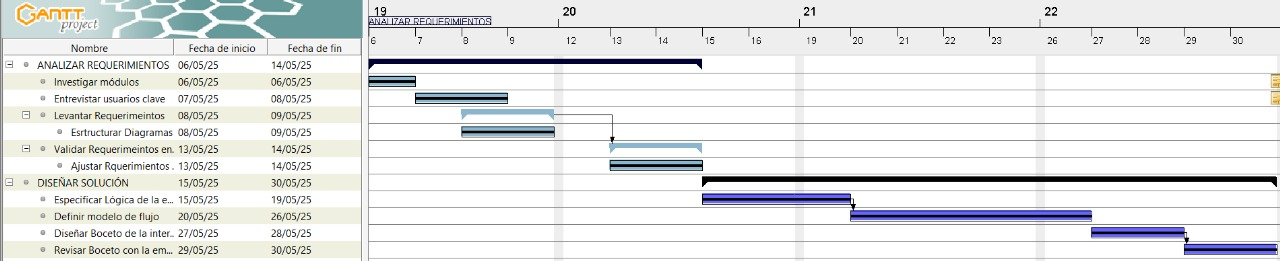
\includegraphics[width=0.9\textwidth]{Gantt_Mayo_30.jpg}
  \caption{Periodo correspondientes a Mayo}\label{a03}
\end{figure}

\begin{figure}[htp]
  \centering
  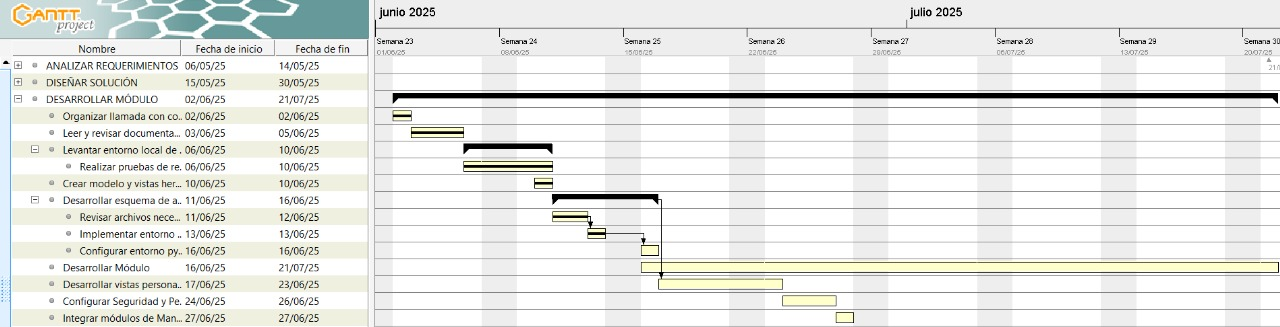
\includegraphics[width=0.9\textwidth]{Gantt_Week_23_30.jpg}
  \caption{Periodo correspondiente a Junio-Julio}\label{a04}
\end{figure}

\begin{figure}[htp]
  \centering
  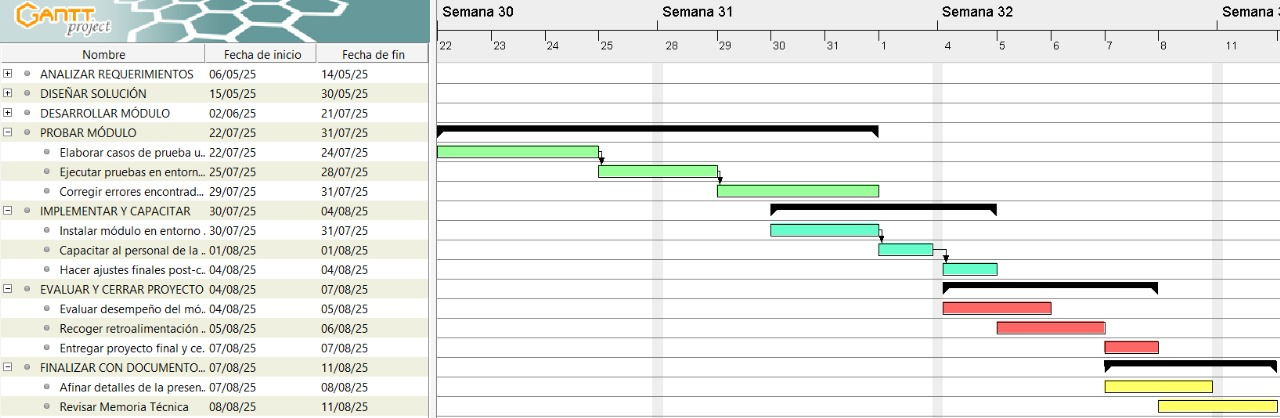
\includegraphics[width=0.9\textwidth]{Gantt_Week_30_32.jpg}
  \caption{Periodo correspondiente a Julio-Agosto}\label{a05}
\end{figure}
%CAPITULO MARCO TEÓRICO: bases teorícas del proyecto. conceptos básicos y antecedentes o información existente.
%____________________________________________________________________________________________________________________

% ==========================================================
%       INICIO DEL CAPÍTULO 4: MARCO TEÓRICO (VERSIÓN FINAL ACTUALIZADA)
% ==========================================================

\chapter{Marco Teórico}
\label{chap:marco_teorico}

Para comprender la construcción de este proyecto desde su núcleo, este capítulo presenta la información teórica y tecnológica indispensable. Su objetivo es exponer los conceptos que sustentan la solución desarrollada, justificando las decisiones técnicas y metodológicas que se tomaron.

El capítulo se enfoca en la arquitectura desacoplada y las tecnologías seleccionadas: \textbf{React} como librería para la interfaz de usuario, \textbf{Vite} como herramienta para optimizar el desarrollo y \textbf{Node.js} como el entorno para el servidor. Se inicia con una breve contextualización del entorno empresarial basado en sistemas ERP para fundamentar la pertinencia del proyecto.

\subsection{Metodología: Modelo en cascada}


Para el proceso de desarrollo de este proyecto se empleó una metodología en cascada, la cual y según el articulo \textit{Modelos de Desarrollo de software} realizado por \citet{DOLIVERA2021} para la \textbf{Revista Cubana de Ciencias Informáticas} consta de 5 etapas que son representadas en fases qué, si bien se mantienen separadas del proceso, son dependientes una de la anterior puesto que una fase no puede iniciarse sin antes terminarse y aprobarse la anterior de paso realizando correcciones de problemas detectados en fases previas. A continuación se presenta la figura (\ref{CASCADA}) donde se muestra como interactúan las fases entre sí además de una breve explicación de cada fase.

\begin{figure} [H]
  \centering
  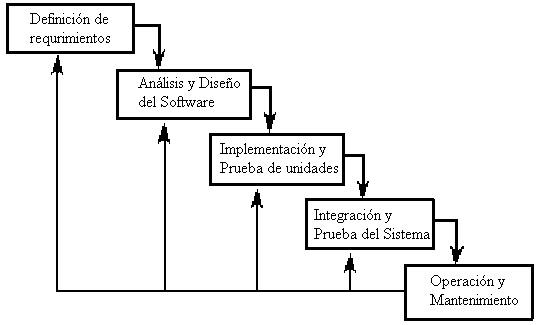
\includegraphics[width=0.9\textwidth]{CASCADA.jpg}
  \caption{Interacción de las fases en el modelo cascada}\label{CASCADA}
\end{figure}

\begin{itemize}
  \item \textbf{Levantamiento/Definición de Requisitos:}Los servicios, restricciones y objetivos son establecidos con los usuarios del sistema. Se busca hacer esta definición en detalle.
  \item \textbf{Diseño de Sistema y Software:}Se particiona en sistemas de software o hardware. Se establece la arquitectura total del sistema. Se identifican y describen las abstracciones y relaciones de los componentes del sistema.
  \item \textbf{Implementación y Pruebas Unitarias:}Construcción de los módulos y unidades de software. Se realizan pruebas de cada unidad.
  \item \textbf{Integración y Pruebas del Sistema:}Se integran todas las unidades, se prueban en conjunto y se entrega el conjunto probado al cliente.
  \item \textbf{Operación y Mantenimiento:} El sistema es puesto en marcha y se realiza la corrección de errores descubiertos. Se realizan mejoras de implementación y se identifican nuevos requisitos.
\end{itemize}




\section{Contexto y justificación de la arquitectura}
\label{sec:contexto_justificacion}

La problemática que aborda este proyecto surge dentro de una empresa cuya gestión operativa se apoya en un sistema de \textbf{Planificación de Recursos Empresariales (ERP)} bajo un modelo de \textbf{Software como Servicio (SaaS)}. Un ERP es una plataforma de software integrado que busca optimizar y centralizar los procesos de negocio de una empresa.

Aunque estos sistemas son potentes, su naturaleza monolítica puede presentar limitaciones. Un estudio realizado por \citet{Correal2021} sobre la implementación de sistemas ERP revela varias desventajas clave que validan la necesidad de soluciones externas y especializadas. Entre las más relevantes se encuentran:
\begin{itemize}
    \item \textbf{Obsolescencia y falta de integración:} Los sistemas ERP pueden presentar una notable falta de integración con herramientas modernas.
    \item \textbf{Procesamiento de datos externo:} Esta falta de integración obliga a los usuarios a recurrir a herramientas externas como Excel.
    \item \textbf{Rigidez ante el cambio:} Se requieren herramientas más dinámicas que se adapten rápidamente a las transformaciones de la empresa.
\end{itemize}
Estas limitaciones,fundamentan la decisión estratégica de optar por una arquitectura desacoplada para este proyecto.

\section{Desarrollo frontend: ecosistema React}
\label{sec:desarrollo_frontend}

La elección de una tecnología para la interfaz de usuario (frontend) es un factor determinante en la usabilidad y el rendimiento. Para este proyecto se seleccionó \textbf{React}, una de las librerías de JavaScript de código abierto más influyentes para la construcción de interfaces interactivas y reutilizables \citep{Murgueytio2022}.

\subsection{Paradigma declarativo y arquitectura basada en componentes}
\label{sec:react_paradigma}

El paradigma de \textbf{React} se fundamenta en una arquitectura basada en \textbf{componentes} y un enfoque \textbf{declarativo}. Permite a los desarrolladores construir interfaces de usuario complejas a partir de piezas de código pequeñas y aisladas. Para ello, se utiliza la extensión de sintaxis \textbf{JSX}, la cual permite escribir una estructura similar a HTML directamente en el código JavaScript. Este enfoque hace que el código sea más predecible, ya que el desarrollador solo necesita describir el estado final de la interfaz, y \textbf{React} se encarga de las actualizaciones de manera eficiente \citep{ReactDocs2025, TaipeQuishpe2022}.

\subsection{El Virtual DOM y su impacto en el rendimiento}
\label{sec:react_vdom}

Una de las innovaciones técnicas de \textbf{React} es el uso de un \textbf{DOM Virtual (VDOM)}. En lugar de manipular directamente el costoso DOM del navegador, \textbf{React} mantiene una copia ligera de su estructura en memoria. Cuando el estado de un componente cambia, un algoritmo de ``diferenciación'' (\textit{diffing}) calcula el conjunto mínimo de cambios necesarios. Finalmente, este proceso de \textbf{reconciliación} aplica únicamente dichas diferencias al DOM real, optimizando drásticamente el rendimiento de la aplicación \citep{TaipeQuishpe2022, ReactDocs2025}.

\subsection{Gestión del estado: de Hooks a gestores globales}
\label{sec:react_hooks}

En \textbf{React}, el \textbf{estado (state)} contiene los datos que describen la condición de un componente. Para gestionar este estado, se introdujeron los \textbf{Hooks}, funciones que permiten ``engancharse'' a las características de \textbf{React} desde componentes funcionales. Los más esenciales son useState y useEffect. Para aplicaciones más complejas, el ecosistema ofrece soluciones de gestión de estado global, como la \textbf{API Context} nativa o librerías como \textbf{Redux}, que proporcionan un almacén centralizado para el estado de toda la aplicación \citep{ReactDocs2025}.

\subsection{Ecosistema y herramientas de construcción: Vite}
\label{sec:vite}
El desarrollo moderno depende de \textbf{herramientas de construcción} (\textit{build tools}). \textbf{Vite} es una herramienta de nueva generación que busca proporcionar una experiencia de desarrollo notablemente más rápida. Su principal ventaja es que aprovecha los \textbf{módulos ES nativos (ESM)} del navegador durante el desarrollo. Para la fase de producción, \textbf{Vite} utiliza internamente el empaquetador Rollup para generar un paquete de código altamente optimizado \citep{ViteDocs2025}.

\section{Arquitectura de la solución: Backend desacoplado}
\label{sec:arquitectura_solucion}
Frente al modelo monolítico de un ERP, una arquitectura desacoplada separa completamente el frontend del backend. La comunicación entre ambas capas se establece a través de una \textbf{API (Interfaz de Programación de Aplicaciones)}, la cual actúa como un ``enlace que posibilita que las aplicaciones se comuniquen entre sí'' \citep{TaipeQuishpe2022}.

\subsection{La API como contrato y el reto de CORS}
\label{sec:api_contrato_cors}
La API define un \textbf{contrato} con un conjunto de reglas y \textbf{endpoints} que el frontend utiliza para solicitar o enviar información. Este proyecto utiliza una \textbf{API REST}, un estilo de arquitectura que usa los verbos del protocolo HTTP y el formato JSON para el intercambio de datos. Un aspecto técnico indispensable en esta arquitectura es el \textbf{Intercambio de Recursos de Origen Cruzado (CORS)}. Por defecto, los navegadores web aplican una ``política del mismo origen'' que restringe las peticiones HTTP a un dominio diferente. Dado que el frontend y el backend operan en orígenes distintos, es crucial que el servidor implemente cabeceras CORS para indicar al navegador que las peticiones desde el frontend están permitidas y son seguras \citep{MDNCorsGuide}.

\subsection{Node.js y Express como entorno para el Backend}
\label{sec:nodejs_express_backend}
Para implementar el backend, este proyecto utiliza \textbf{Node.js}, definido por su documentación oficial como un ``entorno de ejecución de JavaScript asíncrono, impulsado por eventos, diseñado para construir aplicaciones de red escalables'' \citep{NodeDocs2025}. Para facilitar la creación de la API REST, se utilizó \textbf{Express.js}, un framework minimalista y flexible para Node.js. Express simplifica enormemente el manejo de rutas (endpoints), la gestión de peticiones HTTP y la configuración de \textit{middleware} (como el que gestiona CORS), permitiendo construir el backend de manera rápida y organizada \citep{ExpressDocs}.

\subsection{Gestión de la base de datos: Drizzle ORM}
\label{sec:drizzle_orm}
Para la comunicación entre el backend y la base de datos PostgreSQL, se utilizó \textbf{Drizzle ORM}. Un ORM (Mapeo Objeto-Relacional) es una técnica que permite interactuar con la base de datos usando objetos y clases de un lenguaje de programación, en este caso TypeScript. Drizzle es un ORM ``headless'' o sin cabeza, diseñado para ser ligero, rápido y, sobre todo, totalmente seguro en cuanto a tipos (\textit{typesafe}). A diferencia de otros ORMs, no abstrae por completo el lenguaje SQL, sino que proporciona un constructor de consultas que refleja la sintaxis de SQL, dando al desarrollador el control total sobre las consultas que se ejecutan y garantizando que los resultados sean compatibles con los tipos definidos en TypeScript \citep{DrizzleOrmDocs}.

\subsection{Universalidad de las Convenciones}
\label{sec:convenciones_scala}

La adopción de una convención de nomenclatura no es exclusiva del ecosistema de JavaScript o TypeScript, sino una práctica fundamental en la ingeniería de software en general. Para ilustrar su universalidad, se puede tomar como referencia la guía de estilo oficial del lenguaje de programación Scala, una tecnología robusta utilizada para construir sistemas de alto rendimiento.

En su documentación, se especifica una clara distinción en el uso de las capitales: se debe utilizar \textbf{UpperCamelCase} para nombrar clases y \textit{traits} (un concepto similar a las interfaces), mientras que para nombrar métodos y valores (variables y constantes) se debe utilizar \textbf{lowerCamelCase}. Esta distinción sistemática es crucial, ya que permite a cualquier programador identificar de un vistazo la naturaleza de un identificador dentro del código, mejorando drásticamente la legibilidad y reduciendo la carga cognitiva \citep{ScalaStyleGuide}.

Este ejemplo demuestra que, a pesar de las diferencias sintácticas entre lenguajes, la necesidad de un código limpio y consistente lleva a la adopción de convenciones compartidas, validando la decisión de seguir un estándar estricto en este proyecto.

\subsection{Git, Github y manejo de versiones}
\label{sec:git}
En el contexto del desarrollo de software moderno, el control de versiones se ha convertido en una práctica fundamental para mantener la integridad y la trazabilidad del código fuente. Dos de las herramientas más representativas en este ámbito son \textbf{Git} y \textbf{GitHub}.

\textbf{Git} es un sistema de control de versiones distribuido, diseñado para registrar los cambios realizados en archivos y coordinar el trabajo entre múltiples personas. Fue creado por Linus Torvalds en 2005 con el objetivo de ser rápido, eficiente y confiable, especialmente en proyectos de gran escala como el núcleo de Linux. A diferencia de otros sistemas centralizados, Git permite que cada desarrollador tenga una copia completa del historial del proyecto, lo que facilita el trabajo offline y reduce el riesgo de pérdida de información \cite{progit}.

\textbf{GitHub}, por su parte, es una plataforma de desarrollo colaborativo basada en la nube que utiliza Git como motor de control de versiones. Permite a los desarrolladores alojar repositorios de código, colaborar mediante solicitudes de extracción (\textit{pull requests}), realizar seguimiento de problemas (\textit{issues}) y automatizar flujos de trabajo a través de integraciones y acciones. GitHub ha ganado popularidad no solo por su interfaz amigable, sino también por ofrecer herramientas que mejoran la productividad y la colaboración entre equipos distribuidos \cite{githubdocs}.

De acuerdo con la documentación oficial de GitHub, ``GitHub es una plataforma de desarrollo colaborativo que permite almacenar y gestionar código, así como realizar un seguimiento de los cambios y colaborar con otros usuarios''. Esta sinergia entre Git como tecnología subyacente y GitHub como servicio de alojamiento y colaboración ha sido clave en la adopción de buenas prácticas en la ingeniería de software moderna \cite{githubdocs}.



%\section{Calidad y Pruebas en Aplicaciones Modernas}
%\label{sec:calidad_pruebas}
%La construcción de software no finaliza con la escritura del código; es fundamental asegurar su calidad a través de un proceso de pruebas estructurado.
%
%%\subsection{Tipos de Pruebas de Software}
%%El aseguramiento de la calidad (QA) implica diferentes niveles de pruebas. Las \textbf{pruebas unitarias} verifican componentes de código de forma aislada. Las \textbf{pruebas de integración} comprueban que varios componentes interactúen correctamente. Finalmente, las \textbf{pruebas de extremo a extremo (E2E)} simulan el flujo completo de un usuario real en la aplicación.
%%
%%\subsection{Automatización de Pruebas en el Frontend}
%%Realizar pruebas manualmente es un proceso lento y propenso a errores. Por ello, la \textbf{automatización de pruebas} es una práctica indispensable. Como se detalla en el estudio de \citet{Murgueytio2022}, el desarrollo de frameworks de pruebas automatizadas permite ejecutar casos de uso de manera repetida y consistente, asegurando la calidad sin sacrificar la velocidad.


% ==========================================================
%        FIN DEL CAPÍTULO 4: MARCO TEÓRICO (VERSIÓN FINAL ACTUALIZADA)
% ==========================================================



\chapter{Desarrollo del Proyecto}
\newpage



\section{Requerimientos}


%\subsection{Requerimientos funcionales y no funcionales}


La fase de levantamiento de requerimientos es el pilar fundamental de cualquier proyecto de software, ya en ella se definen las capacidades y condiciones que la solución final debe cumplir. En esta sección, se detallan formalmente dichas condiciones, las cuales fueron recopiladas a partir del análisis de la problemática y las necesidades de la empresa.

Para una mayor claridad, los requerimientos se han clasificado en dos categorías: Requerimientos Funcionales, que describen qué debe hacer el sistema, y Requerimientos No Funcionales, que definen cómo debe ser el sistema en términos de calidad y operación. Ambas categorías se pueden consultar en los cuadros  \ref{tab:rf001} al \ref{tab:rf010} para los requerimientos funcionales y en los cuadros \ref{tab:rnf001} al \ref{tab:rnf003} para los no funcionales.

% --- Requerimiento RF-001 ---
\begin{table}[H]
    \centering
    \caption{Requerimiento Funcional: Registro de Solicitudes}
    \label{tab:rf001}
    \begin{tabular}{ll}
        \toprule
        \textbf{ID} & RF-001 \\
        \textbf{Nombre} & Registro de Solicitudes \\
        \textbf{Tipo} & Requerimiento Funcional \\
        \textbf{Prioridad} & Alta \\
        \midrule
        \multicolumn{2}{l}{
            \parbox{0.9\linewidth}{
                \textbf{Descripción:} El sistema debe proporcionar un formulario intuitivo para que usuarios autorizados registren nuevas solicitudes de reproceso o reparación. El formulario debe validar los campos obligatorios antes de guardar y mostrar confirmación al usuario. Debe integrarse con el módulo de autenticación para identificar automáticamente al solicitante.
            }
        } \\
        \bottomrule
    \end{tabular}
\end{table}

% --- Requerimiento RF-002 ---
\begin{table}[H]
    \centering
    \caption{Requerimiento Funcional: Generación Automática de Folios}
    \label{tab:rf002}
    \begin{tabular}{ll}
        \toprule
        \textbf{ID} & RF-002 \\
        \textbf{Nombre} & Generación Automática de Folios \\
        \textbf{Tipo} & Requerimiento Funcional (Reglas de negocio) \\
        \textbf{Prioridad} & Alta \\
        \midrule
        \multicolumn{2}{l}{
            \parbox{0.9\linewidth}{
                \textbf{Descripción:} Cada nueva solicitud debe generar un folio único con el formato: JN-REQ-MM-AA-CCC, donde: JN-REQ es prefijo fijo, MM-AA representa el mes y año actual, y CCC es un contador consecutivo de 3 dígitos que se reinicia mensualmente. El sistema debe garantizar que no existan folios duplicados. Ejemplo: JN-REQ-05-25-042.
            }
        } \\
        \bottomrule
    \end{tabular}
\end{table}

% --- Requerimiento RF-003 ---
\begin{table}[H]
    \centering
    \caption{Requerimiento Funcional: Gestión de Datos de Solicitud}
    \label{tab:rf003}
    \begin{tabular}{ll}
        \toprule
        \textbf{ID} & RF-003 \\
        \textbf{Nombre} & Gestión de Datos de Solicitud \\
        \textbf{Tipo} & Requerimiento Funcional (Gestión de datos) \\
        \textbf{Prioridad} & Alta \\
        \midrule
        \multicolumn{2}{l}{
            \parbox{0.9\linewidth}{
                \textbf{Descripción:} Las solicitudes deben almacenar: Fecha de solicitud (Autogenerada), Solicitante (Obtenido del usuario autenticado), Área (Lista desplegable), Estado (Flujo definido), Costes (Campo restringido), Fecha de entrega (Editable), Tiempo total (Calculado) y Observaciones (Texto libre).
            }
        } \\
        \bottomrule
    \end{tabular}
\end{table}

% --- Requerimiento RF-004 ---
\begin{table}[H]
    \centering
    \caption{Requerimiento Funcional: Seguimiento de Reparación}
    \label{tab:rf004}
    \begin{tabular}{ll}
        \toprule
        \textbf{ID} & RF-004 \\
        \textbf{Nombre} & Seguimiento de Reparación (Registro de procesos) \\
        \textbf{Tipo} & Requerimiento Funcional \\
        \textbf{Prioridad} & Media \\
        \midrule
        \multicolumn{2}{l}{
            \parbox{0.9\linewidth}{
                \textbf{Descripción:} Para cada etapa del reproceso, el sistema debe permitir registrar: el área donde se realiza la operación, el operador implicado, el supervisor encargado, la fecha (autogenerada) y las horas de inicio y fin con validación. Los registros deben vincularse a la solicitud principal.
            }
        } \\
        \bottomrule
    \end{tabular}
\end{table}

% --- Requerimiento RF-005 ---
\begin{table}[H]
    \centering
    \caption{Requerimiento Funcional: Registro Múltiple de Piezas}
    \label{tab:rf005}
    \begin{tabular}{ll}
        \toprule
        \textbf{ID} & RF-005 \\
        \textbf{Nombre} & Registro Múltiple de Piezas \\
        \textbf{Tipo} & Requerimiento Funcional (Entrada de datos) \\
        \textbf{Prioridad} & Alta \\
        \midrule
        \multicolumn{2}{l}{
            \parbox{0.9\linewidth}{
                \textbf{Descripción:} El sistema debe permitir agregar N piezas a una solicitud mediante un botón Añadir pieza que muestre un subformulario. Cada pieza debe guardarse individualmente y asociarse al folio de la solicitud padre. El usuario debe poder editar o eliminar piezas antes de finalizar el proceso.
            }
        } \\
        \bottomrule
    \end{tabular}
\end{table}

% --- Requerimiento RF-006 ---
\begin{table}[H]
    \centering
    \caption{Requerimiento Funcional: Detalles de Piezas}
    \label{tab:rf006}
    \begin{tabular}{ll}
        \toprule
        \textbf{ID} & RF-006 \\
        \textbf{Nombre} & Detalles de Piezas \\
        \textbf{Tipo} & Requerimiento Funcional (Gestión de datos) \\
        \textbf{Prioridad} & Alta \\
        \midrule
        \multicolumn{2}{l}{
            \parbox{0.9\linewidth}{
                \textbf{Descripción:} Cada pieza debe contener: No. Solicitud (no editable), Modelo/Tela/Color (con autocompletado), Tipo de pieza (desplegable), Descripción del daño (obligatorio, con opción para adjuntar imágenes) y Responsable (opcional).
            }
        } \\
        \bottomrule
    \end{tabular}
\end{table}

% --- Requerimiento RF-007 ---
\begin{table}[H]
    \centering
    \caption{Requerimiento Funcional: Aprobación/Rechazo por Supervisor}
    \label{tab:rf007}
    \begin{tabular}{ll}
        \toprule
        \textbf{ID} & RF-007 \\
        \textbf{Nombre} & Aprobación/Rechazo por Supervisor \\
        \textbf{Tipo} & Requerimiento Funcional (Flujo de trabajo) \\
        \textbf{Prioridad} & Media \\
        \midrule
        \multicolumn{2}{l}{
            \parbox{0.9\linewidth}{
                \textbf{Descripción:} Los supervisores deben recibir notificaciones de solicitudes En revisión. Desde su panel, podrán aprobar (cambia estado y notifica) o rechazar (requiere una razón obligatoria). Todas las acciones se registran en una bitácora.
            }
        } \\
        \bottomrule
    \end{tabular}
\end{table}

% --- Requerimiento RF-008 ---
\begin{table}[H]
    \centering
    \caption{Requerimiento Funcional: Finalización del Proceso}
    \label{tab:rf008}
    \begin{tabular}{ll}
        \toprule
        \textbf{ID} & RF-008 \\
        \textbf{Nombre} & Finalización del Proceso \\
        \textbf{Tipo} & Requerimiento Funcional (Flujo de trabajo) \\
        \textbf{Prioridad} & Alta \\
        \midrule
        \multicolumn{2}{l}{
            \parbox{0.9\linewidth}{
                \textbf{Descripción:} Cuando la última operación se marca como Finalizada, el sistema debe cambiar el estado de la solicitud a Completado, calcular el tiempo total, notificar a los interesados por correo y bloquear las ediciones posteriores (modo solo lectura).
            }
        } \\
        \bottomrule
    \end{tabular}
\end{table}

% --- Requerimiento RF-009 ---
\begin{table}[H]
    \centering
    \caption{Requerimiento Funcional: Autenticación de Usuarios}
    \label{tab:rf009}
    \begin{tabular}{ll}
        \toprule
        \textbf{ID} & RF-009 \\
        \textbf{Nombre} & Autenticación de Usuarios \\
        \textbf{Tipo} & Requerimiento Funcional (Seguridad) \\
        \textbf{Prioridad} & Alta \\
        \midrule
        \multicolumn{2}{l}{
            \parbox{0.9\linewidth}{
                \textbf{Descripción:} El sistema debe requerir inicio de sesión para acceder a sus funcionalidades. Las contraseñas deben almacenarse de forma encriptada y el sistema debe implementar un bloqueo temporal tras 3 intentos de inicio de sesión fallidos.
            }
        } \\
        \bottomrule
    \end{tabular}
\end{table}

% --- Requerimiento RF-010 ---
\begin{table}[H]
    \centering
    \caption{Requerimiento Funcional: Control de Permisos por Roles}
    \label{tab:rf010}
    \begin{tabular}{ll}
        \toprule
        \textbf{ID} & RF-010 \\
        \textbf{Nombre} & Control de Permisos \\
        \textbf{Tipo} & Requerimiento Funcional (Seguridad) \\
        \textbf{Prioridad} & Alta \\
        \midrule
        \multicolumn{2}{l}{
            \parbox{0.9\linewidth}{
                \textbf{Descripción:} El sistema debe gestionar permisos diferenciados por roles: \textbf{Supervisores} (aprobar/rechazar, ver costes), \textbf{Operadores} (registrar solicitudes en su área) y \textbf{Administradores} (CRUD completo de solicitudes y usuarios).
            }
        } \\
        \bottomrule
    \end{tabular}
\end{table}



% --- Requerimiento No Funcional RNF-001 ---
\begin{table}[H]
    \centering
    \caption{Requerimiento No Funcional: Accesibilidad y Compatibilidad}
    \label{tab:rnf001}
    \begin{tabular}{ll}
        \toprule
        \textbf{ID} & RNF-001 \\
        \textbf{Nombre} & Accesibilidad y Compatibilidad \\
        \textbf{Tipo} & Requerimiento No Funcional \\
        \textbf{Prioridad} & Alta \\
        \midrule
        \multicolumn{2}{l}{
            \parbox{0.9\linewidth}{
                \textbf{Descripción:} El sistema debe ser accesible desde cualquier dispositivo con conexión a internet y un navegador web moderno (ej. Chrome, Firefox, Edge).
            }
        } \\
        \bottomrule
    \end{tabular}
\end{table}

% --- Requerimiento No Funcional RNF-002 ---
\begin{table}[H]
    \centering
    \caption{Requerimiento No Funcional: Disponibilidad y Respaldo}
    \label{tab:rnf002}
    \begin{tabular}{ll}
        \toprule
        \textbf{ID} & RNF-002 \\
        \textbf{Nombre} & Disponibilidad y Respaldo \\
        \textbf{Tipo} & Requerimiento No Funcional \\
        \textbf{Prioridad} & Alta \\
        \midrule
        \multicolumn{2}{l}{
            \parbox{0.9\linewidth}{
                \textbf{Descripción:} La base de datos del sistema debe ser respaldada automáticamente al menos una vez al día para garantizar la recuperación de datos en caso de una falla.
            }
        } \\
        \bottomrule
    \end{tabular}
\end{table}

% --- Requerimiento No Funcional RNF-003 ---
\begin{table}[H]
    \centering
    \caption{Requerimiento No Funcional: Usabilidad}
    \label{tab:rnf003}
    \begin{tabular}{ll}
        \toprule
        \textbf{ID} & RNF-003 \\
        \textbf{Nombre} & Usabilidad \\
        \textbf{Tipo} & Requerimiento No Funcional \\
        \textbf{Prioridad} & Alta \\
        \midrule
        \multicolumn{2}{l}{
            \parbox{0.9\linewidth}{
                \textbf{Descripción:} La interfaz de usuario debe ser intuitiva y fácil de usar, permitiendo que el personal con conocimientos básicos de computación pueda operar el sistema eficientemente con un mínimo de capacitación.
            }
        } \\
        \bottomrule
    \end{tabular}
\end{table}







\section{Análisis y Diseño}

\subsection{Elección de la arquitectura: aplicación externa vs. módulo integrado}
\label{sec:eleccion_arquitectura}

Tras el levantamiento y análisis de requerimientos, se procedió a la fase de diseño, donde la decisión más estratégica fue la elección de la arquitectura de software. Inicialmente, la solución más directa aparentaba ser el desarrollo de un módulo integrado directamente en la plataforma \texttt{Odoo}, dado que es el ERP en uso por la empresa. Esta opción, en teoría, permitiría centralizar la operación y aprovechar la infraestructura existente.

Sin embargo, un análisis más profundo reveló una serie de restricciones técnicas y operacionales que hacían de esta alternativa una vía no óptima para el proyecto. Como se menciona en la descripción del proyecto, existían "...restricciones del propio ERP y cuestiones a nivel operacional...". Estas se pueden detallar en los siguientes puntos:

\begin{itemize}
    \item \textbf{Restricciones de interfaz de usuario (UX):} Se estableció como requisito la creación de una experiencia de usuario altamente especializada, fluida y dinámica. Lograr este nivel de interactividad con el framework nativo de \texttt{Odoo} (\texttt{OWL}) habría supuesto una curva de aprendizaje y una complejidad de desarrollo significativamente mayores en comparación con librerías de vanguardia como \texttt{React}, diseñada específicamente para este propósito.

    \item \textbf{Flexibilidad y ciclo de desarrollo:} El desarrollo de un módulo integrado está fuertemente acoplado a los ciclos y versiones de \texttt{Odoo}. El desarrollo de una aplicación externa permitía un ciclo de vida independiente, facilitando actualizaciones y mantenimientos futuros sin afectar la estabilidad del ERP principal.

%    \item \textbf{Restricciones de acceso y despliegue:} Durante la fase de análisis, se identificó que las políticas administrativas de la empresa para garantizar la estabilidad del ERP limitaban el acceso para el despliegue de nuevos módulos de terceros, lo que representaba un riesgo para el cumplimiento de los plazos del proyecto.
\end{itemize}

En virtud de estas limitaciones, se tomó la decisión estratégica de optar por una \textbf{arquitectura desacoplada}. Se determinó que el desarrollo de una herramienta externa, utilizando un stack tecnológico moderno con \texttt{React} en el frontend y \texttt{Node.js} en el backend, era la solución más eficiente y robusta. 




\subsection{Modelo relacional}
El diseño bien logrado de una base de datos es el pilar fundamental en la arquitectura de un sistema, pues es con esto que se define el cómo se almacenará y organizará la información Para este proyecto, se ha utilizado el sistema gestor de bases de datos relacional PostgreSQL, por su robustez y compatibilidad con el ecosistema de Node.js. El siguiente modelo relacional (Figura \ref{ER}) ilustra la estructura diseñada, mostrando las tablas principales y las relaciones que garantizan la integridad de los datos.
\begin{figure}[H]
  \centering
  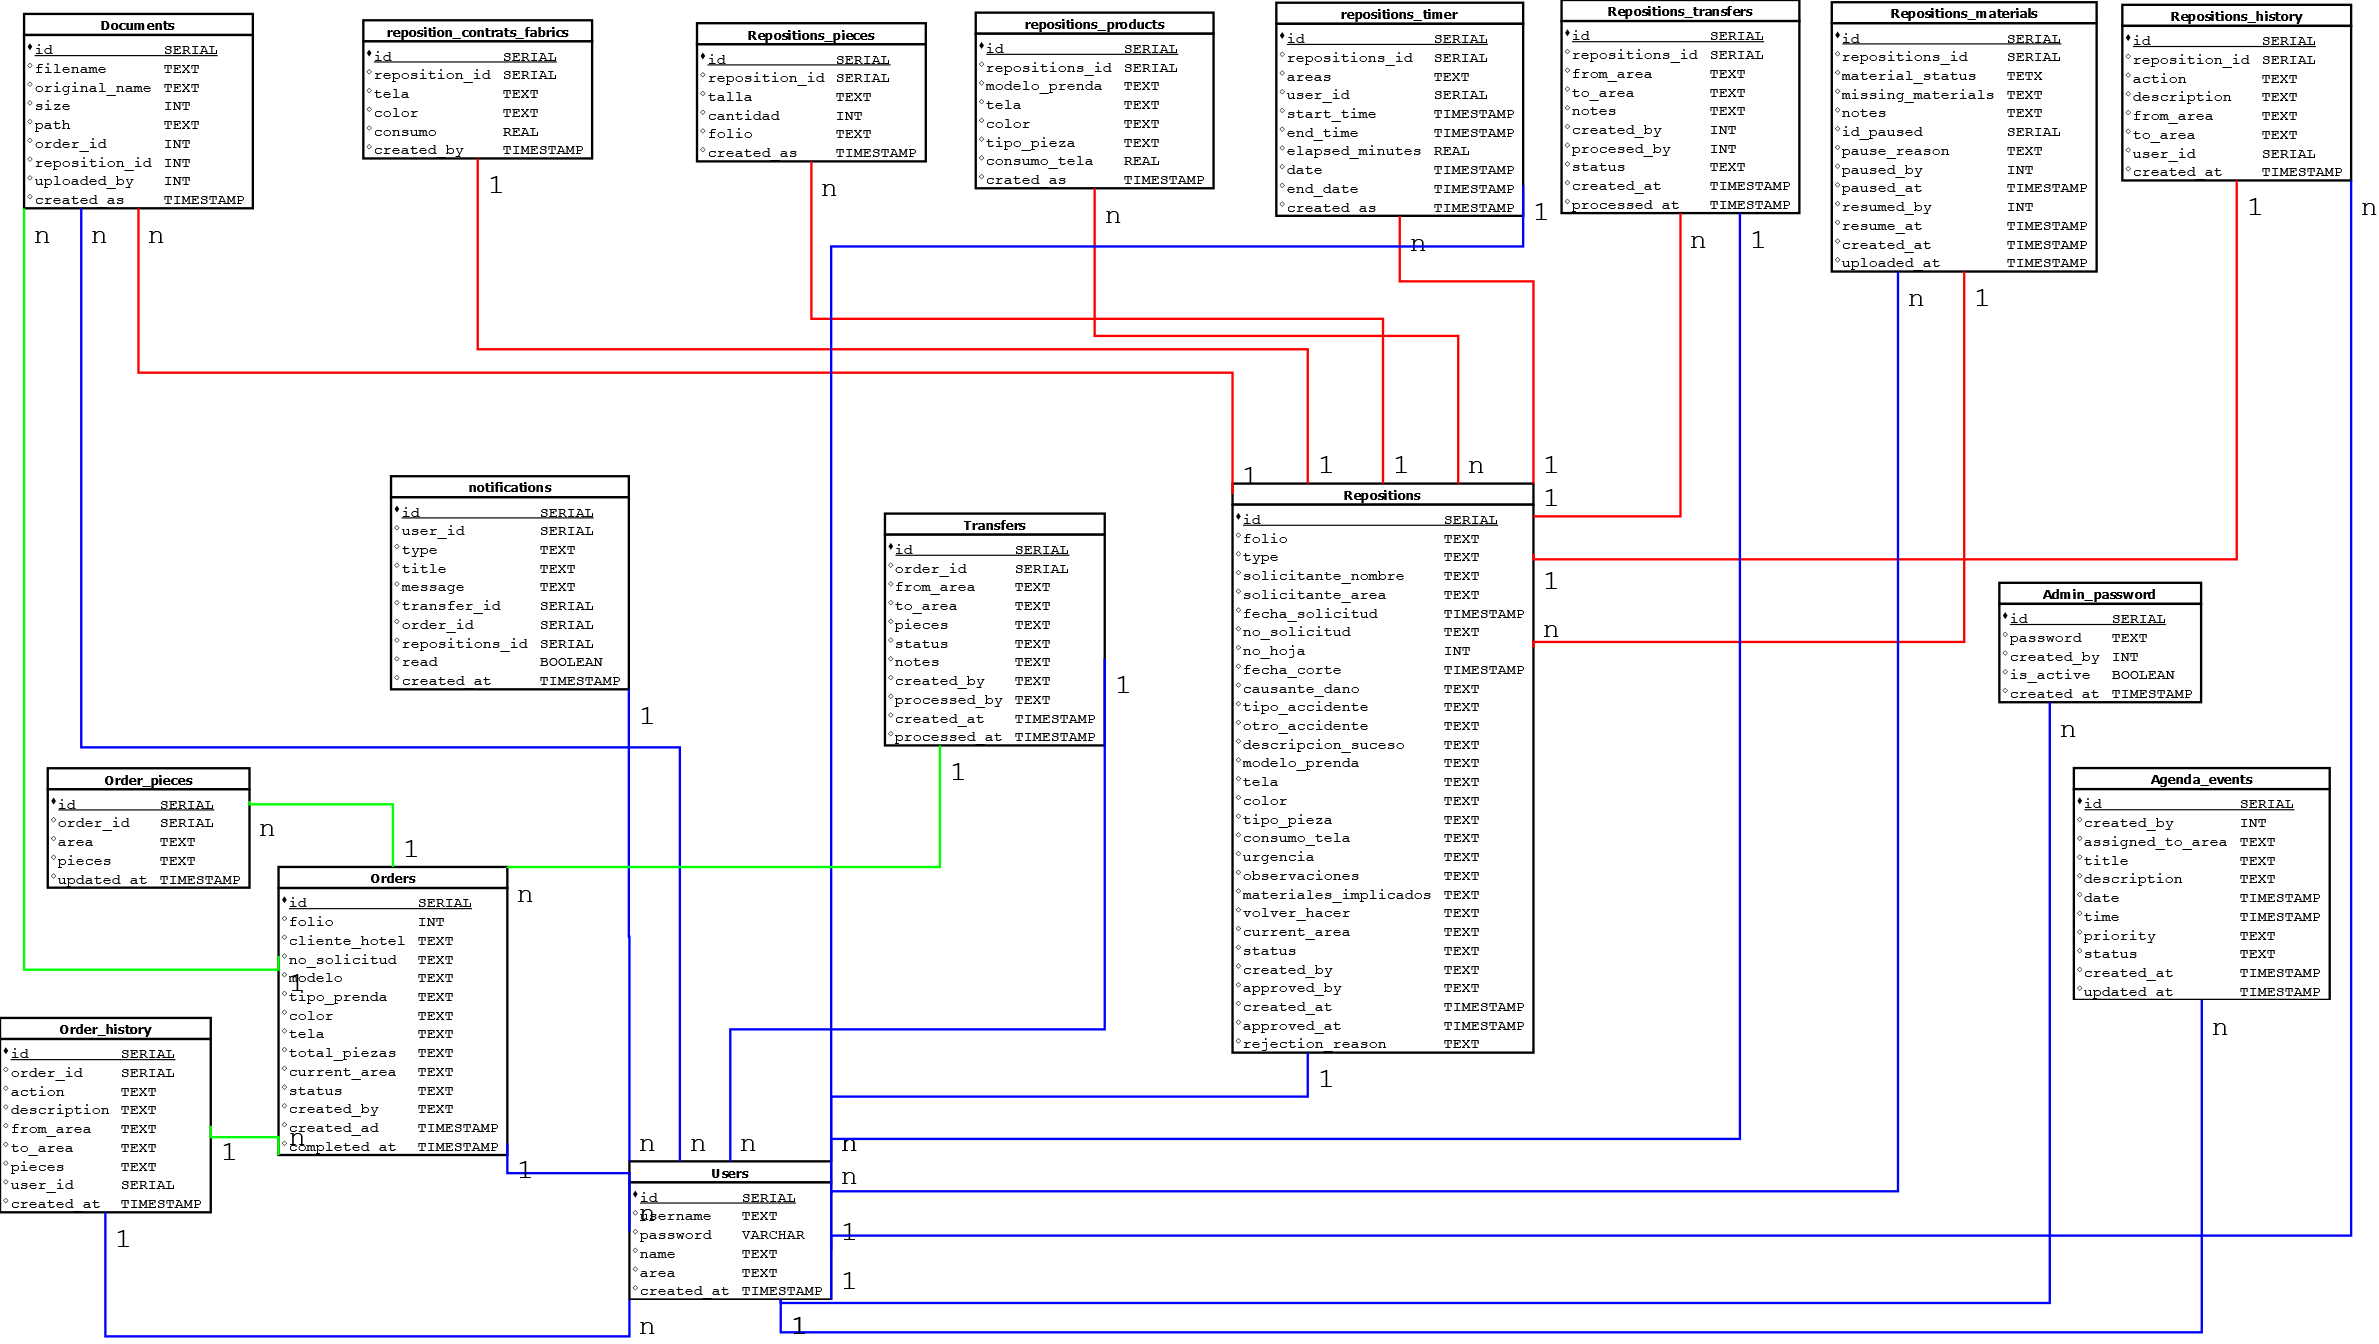
\includegraphics[width=1\textwidth]{Diagrama1.png}
  \caption{Modelo relacional de la base de datos.}\label{ER}
\end{figure} 
 
 \subsection{Casos de uso}
A continuación se presenta los casos de uso y los diagramas (figuras \ref{d01} a \ref{d06}) relacionados a los mismos casos que se identificaron en base a los requerimientos para el desarrollo de esta solución tecnológica y qué, a su vez, ayudaron a comprender de mejor manera la construcción del sistema. 


\begin{itemize}
    \item \textbf{Caso de Uso 001: Registrar Nueva Solicitud} 
    Permite a los Supervisores de área crear nuevas solicitudes de reproceso , generando un folio único de forma automática.
    
\begin{figure}[H]
  \centering
  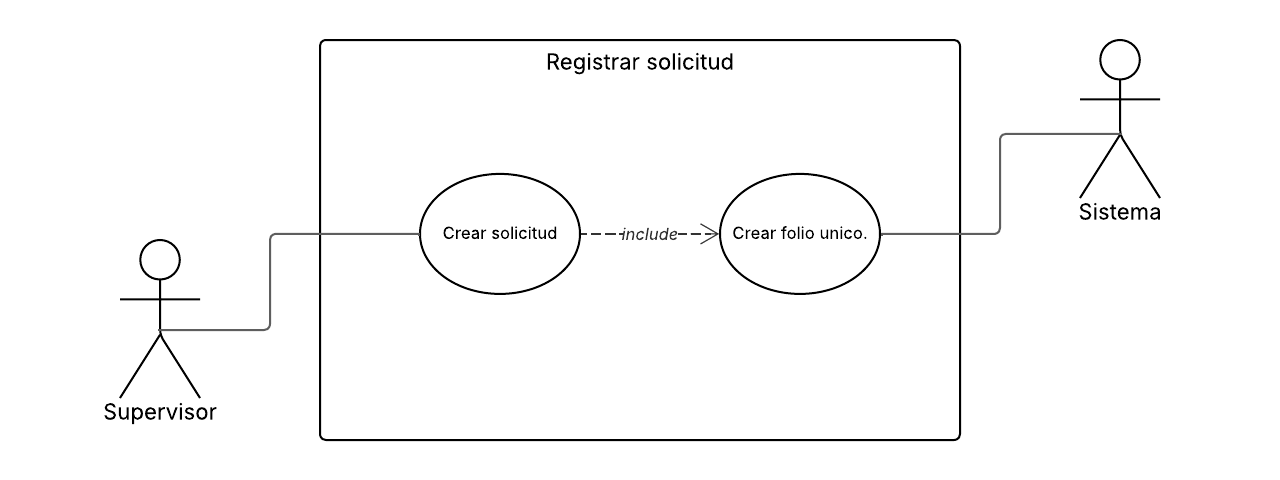
\includegraphics[width=0.8\textwidth]{DIACU01 (1).png}
  \caption{Diagrama de Caso de Uso 001: Registrar Solicitud}\label{d01}
\end{figure}

    \item \textbf{Caso de Uso 002: Registrar Piezas en Solicitud} 
    Permite a Operadores y Administradores añadir, editar o eliminar múltiples piezas  detallando el daño en una solicitud.
    
    \begin{figure}[H]
  \centering
  \hspace*{-3.5 cm}
  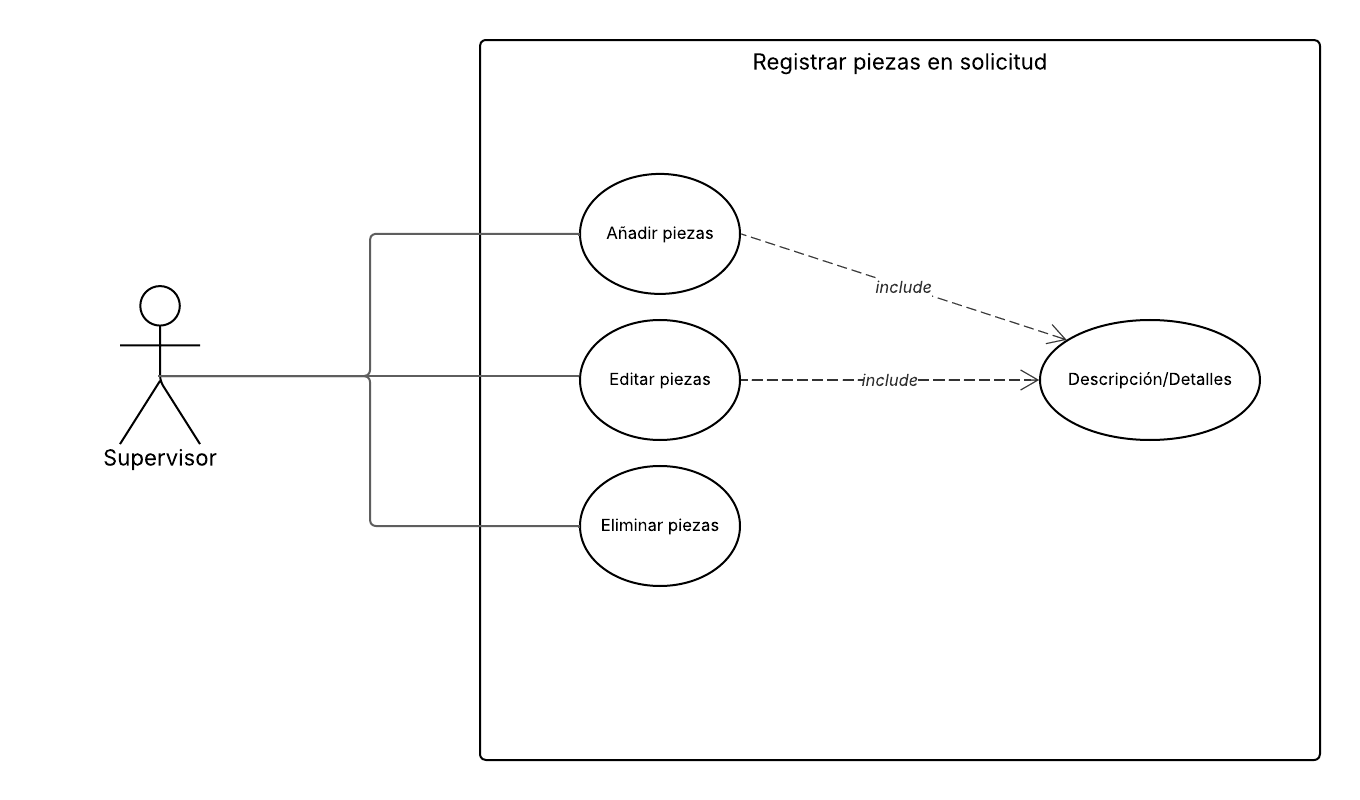
\includegraphics[width=0.7\textwidth]{DIACU02.png}
  \caption{Diagrama de Caso de Uso 002: Registrar Piezas en Solicitud}\label{d02}
\end{figure}
        
    \item \textbf{Caso de Uso 003: Aprobar o Rechazar Solicitud}
    Permite al Supervisor aprobar o rechazar las solicitudes que se encuentran \textbf{En revisión}, registrando una justificación obligatoria en caso de rechazo.

    \begin{figure}[H]
  \centering
  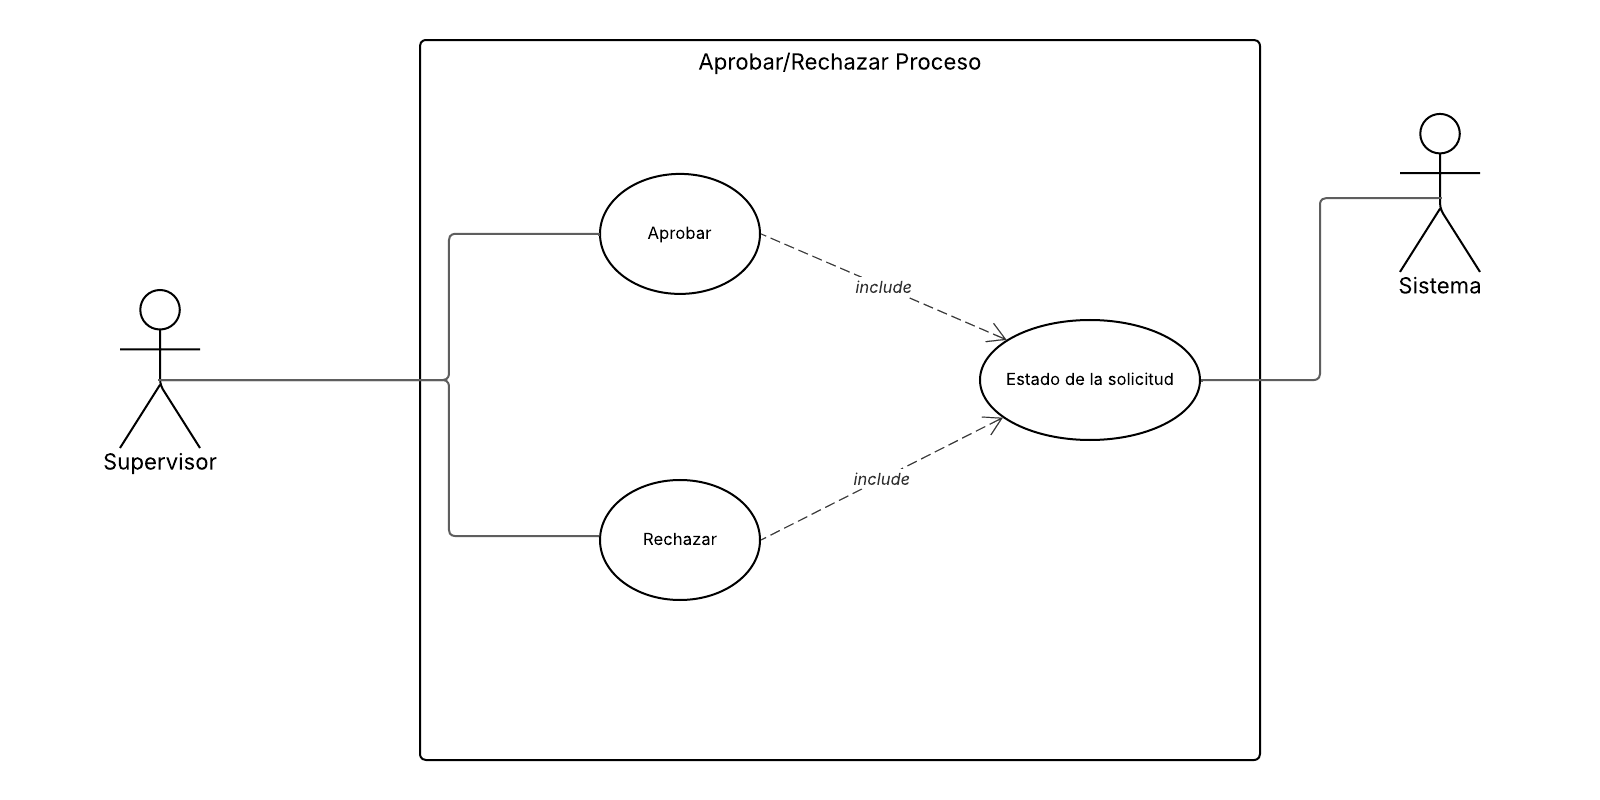
\includegraphics[width=0.9\textwidth]{DIACU03.png}
  \caption{Diagrama de Caso de Uso 003: Aprobar/Rechazar Proceso }\label{d03}
\end{figure}


    \item \textbf{Caso de Uso 004: Finalización de Reproceso}
    Permite al Supervisor marcar la última operación como terminada para cambiar el estado de la solicitud a \textbf{Completado}, notificando a los involucrados y bloqueando ediciones futuras.

    \begin{figure}[H]
  \centering
  \hspace*{-5 cm}
  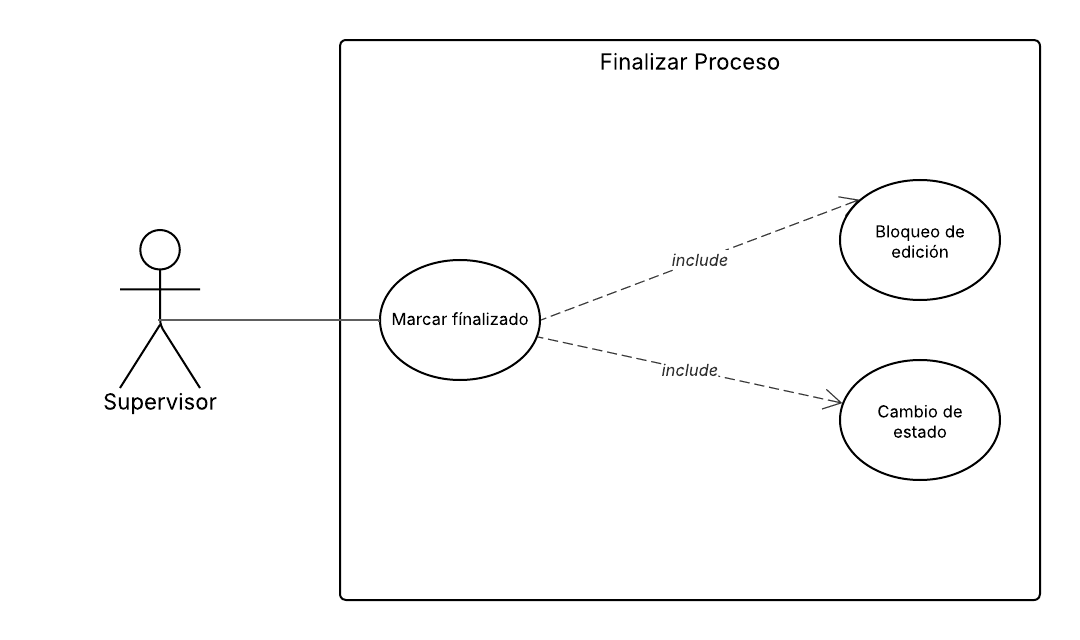
\includegraphics[width=0.7\textwidth]{DIACU04.png}

  \caption{Diagrama de Caso de Uso 004: Finalizar Proceso}\label{d04}
\end{figure}



    \item \textbf{Caso de Uso 005: Registrar Avance de Reparación} 
    Permite al Supervisor registrar el avance, los tiempos y el operador de cada etapa del reproceso.

    \begin{figure}[H]
  \centering
  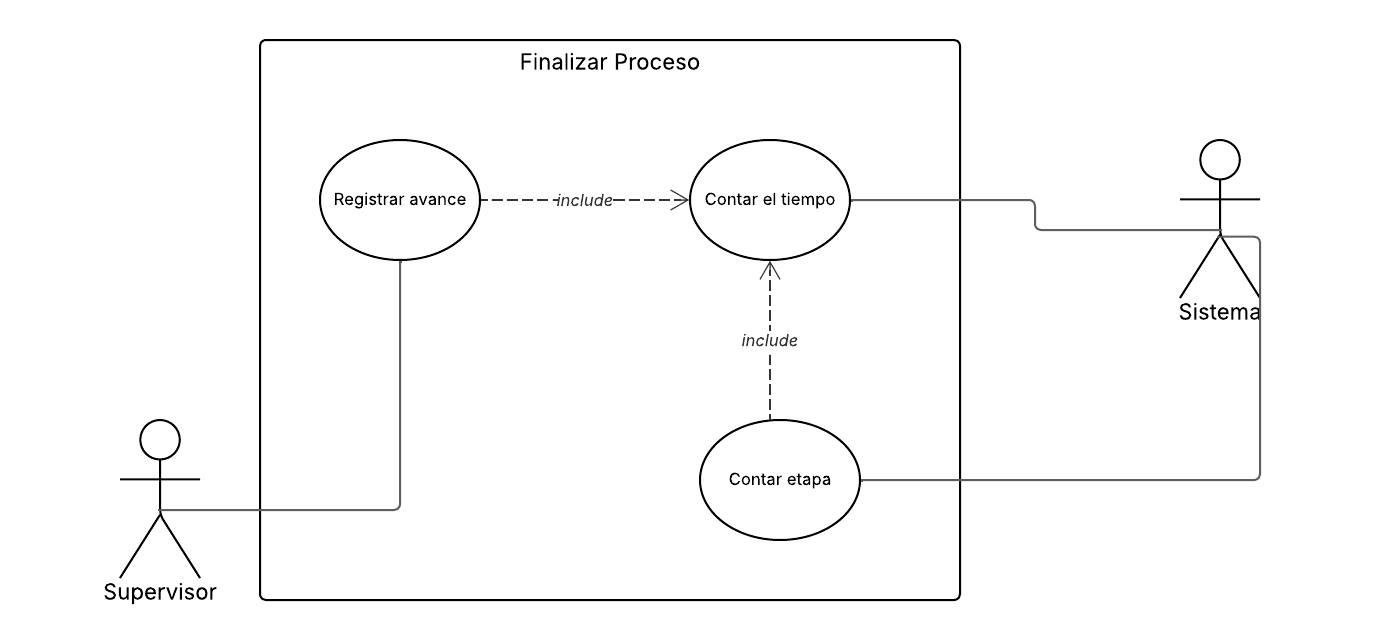
\includegraphics[width=0.9\textwidth]{DIACU05.png}
  \caption{Diagrama de Caso de Uso 005: Registrar Avance}\label{d05}
\end{figure}


    \item \textbf{Caso de Uso 006: Autenticarse en el Sistema} 
    Requiere que todos los usuarios inicien sesión para acceder a las funcionalidades permitidas para su rol.



\begin{figure}[H]
  \centering
  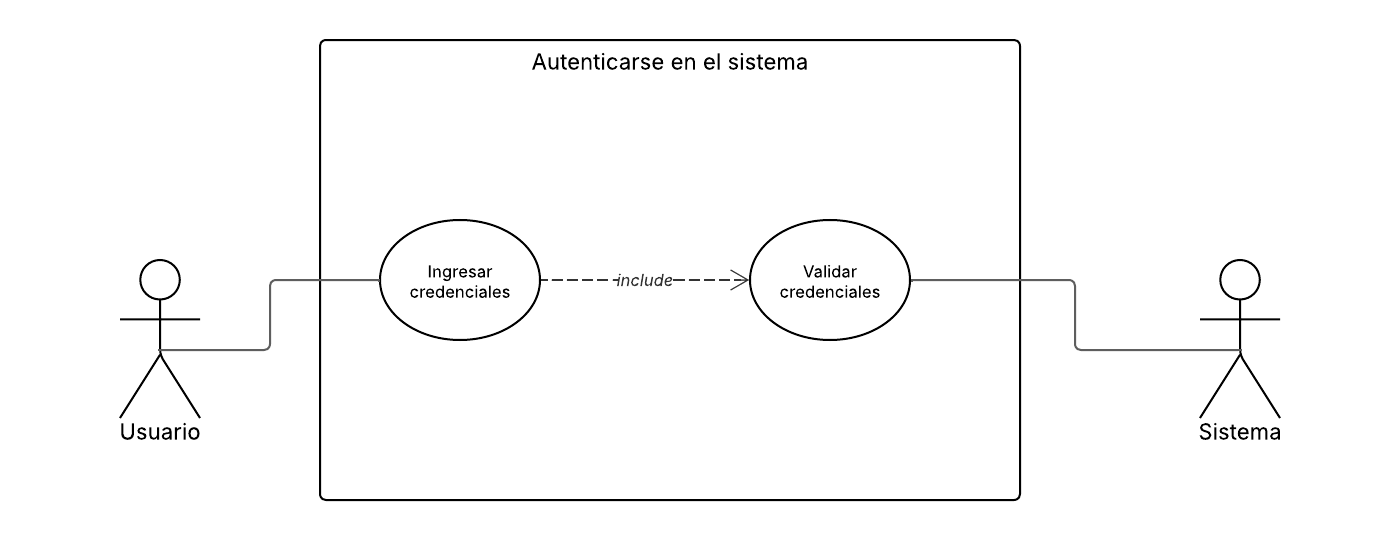
\includegraphics[width=0.9\textwidth]{DIACU06.png}
  \caption{Diagrama de Caso de Uso 006: Autenticarse en el Sistema}\label{d06}
\end{figure}

   % \item \textbf{Caso de Uso 007: Gestionar Permisos de Usuario} 
%    Permite al Administrador gestionar los usuarios y sus permisos de acceso a las distintas funciones del sistema desde un panel centralizado.

\end{itemize}
\section{Desarrollo y elaboración}
Una vez finalizados el levantamiento de requerimientos, esctroctura del modelo relacional de la base de datos y la elección del diseño de la aplicación web, realzamos una junta para discutir los temas de esctroctura de archivos para el desarrollo del proyecto, así mismo las tecnologías que implementariamos tanto en el backend cómo en el frontend, una vez decidos estos pasos empezamos con la elaboración del proyecto.

\subsection{Tecnologías y Entorno de Desarrollo}
\label{sec:tecnologias_entorno}

La elaboración del proyecto se realizó utilizando el siguiente conjunto de tecnologías y herramientas:
\begin{itemize}
    \item \textbf{Frontend:} React.js (v18.2), Vite.
    \item \textbf{Backend:} Node.js (v20.10), Express.js.
    \item \textbf{Base de Datos:} PostgreSQL (v17.5).
    \item \textbf{Control de Versiones:} Git, GitHub.
    \item \textbf{Editor de Código:} Visual Studio Code.
\end{itemize}

%\citep{LinuxMintWebsite, Verdesoto2022Linux}.
Se realizarón las instalaciones correspondientes, la preparación del entorno para que todas las tecnologías trabajaran de manera síncrona y las pruebas correspondientes para descartar incompatibilidades entre las mismas.

\subsection{Estructura de Archivos}
El sistema de gestión de reposiciones JASANA implementa una arquitectura Full-Stack separada con las siguientes divisiones principales:
\vspace{1em}

\textbf{Frontend (/client)}
    \begin{itemize}
    \item \textbf {Framework:} React + TypeScript con Vite
    \item \textbf {Componentes:} Organizados por funcionalidad (orders, repositions, layout, ui)
    \item \textbf {Páginas:} Dashboard, autenticación, órdenes, reposiciones, métricas y administración
    \item \textbf {Características:} PWA, tema oscuro/claro, componentes reutilizables
    \end{itemize}
    
\textbf{Backend (/server)}
\begin{itemize}
    \item \textbf{Servidor:} Express.js + TypeScript
    \item \textbf{Módulos:} Autenticación, rutas API, base de datos, almacenamiento y subida de archivos
    \item \textbf{Middleware:} Conversión camelCase para consistencia de datos
\end{itemize}

\textbf{Base de Datos (/drizzle, /shared)}
\begin{itemize}
    \item \textbf{ORM:} Drizzle con PostgreSQL
    \item \textbf{Esquemas:} Tipos compartidos entre frontend y backend
    \item \textbf{Migraciones:} Control de versiones de la estructura de datos
\end{itemize}

\textbf{Archivos de Configuración}
\begin{itemize}
    \item \textbf{Vite:} Bundling y desarrollo del frontend
    \item \textbf{TypeScript:} Configuración de tipos
    \item \textbf{Tailwind:} Sistema de estilos
    \item \textbf{Package.json:} Dependencias y scripts del proyecto
\end{itemize}
Esta estructura permite separación clara de responsabilidades, escalabilidad y mantenimiento eficiente del código, siguiendo patrones modernos de desarrollo web.

\subsection{Estándares y Convenciones de Codificación}
\label{sec:estandares_codigo}

Para garantizar la legibilidad, consistencia y mantenibilidad del código, es una práctica estándar en el desarrollo de software adoptar una \textbf{convención de nomenclatura}. Esta consiste en un conjunto de reglas para nombrar los distintos identificadores (variables, funciones, clases, etc.) dentro de un proyecto.

En el ecosistema de JavaScript y, por extensión, de \textbf{TypeScript}, la convención más extendida y recomendada es \textbf{camelCase}. Esta práctica consiste en escribir los identificadores uniendo palabras sin espacios, donde la primera palabra comienza con minúscula y cada palabra subsecuente comienza con una letra mayúscula (p. ej., \texttt{nombreDeVariable}). Ejemplo de código en la siguiente imagen (Figura \ref{fig:camelcase})

\begin{figure}[H]
    \centering
    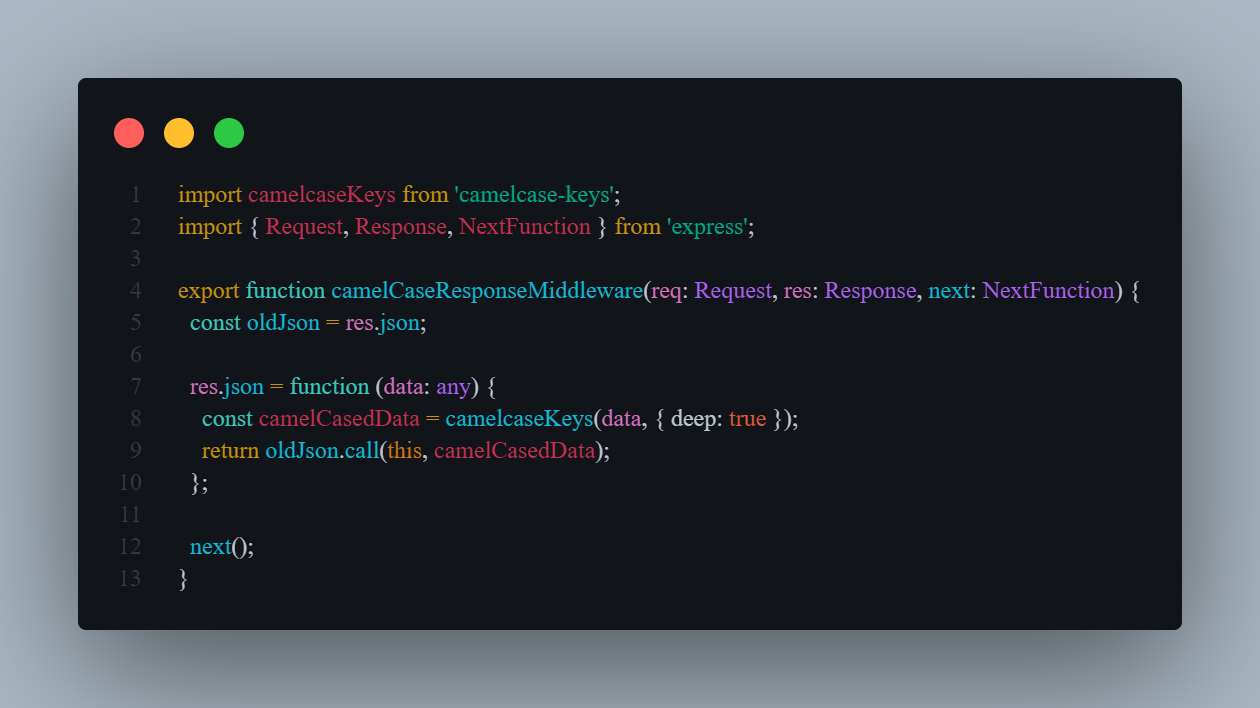
\includegraphics[width=0.9\textwidth]{camelcase.png}
    \caption{Ejemplo de la estructura de CamelCase.}
    \label{fig:camelcase}
\end{figure}

Otros de los elementos que se implementarón al proyecto, fueron los enums, estos se usan para definir un conjunto fijo de valores posibles para una columna. Son útiles cuando necesitas garantizar que un campo solo contenga ciertos valores predefinidos, como un estado o una categoría. Se muestra un ejemplo en la imagen siguiente (Figura \ref{fig:enums})

\begin{figure}[H]
    \centering
    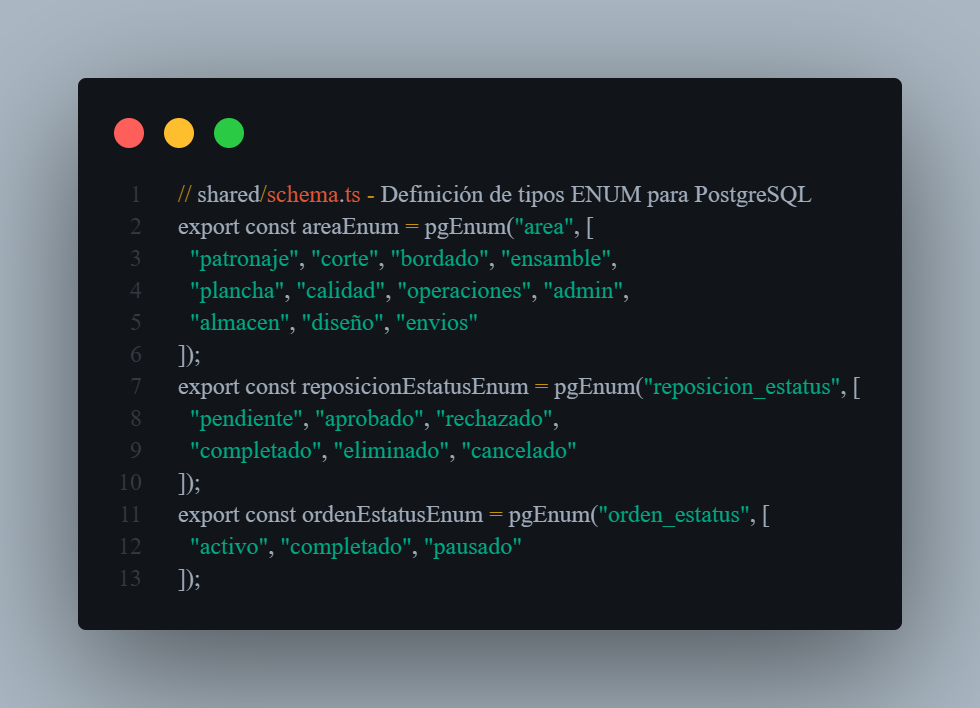
\includegraphics[width=0.9\textwidth]{enums.png}
    \caption{Ejemplo de la estructura de los Enums.}
    \label{fig:enums}
\end{figure}


\subsection{Desarrollo}

\label{sec:evolucion_dashboard}

El componente principal de la aplicación es el Dashboard o Tablero, ya que funciona como el punto central de control para los usuarios. Su diseño no fue estático, sino que evolucionó a través de un proceso de desarrollo iterativo para mejorar la experiencia de usuario y alinear la interfaz con los requerimientos funcionales. A continuación, se muestra esta progresión.

\subsubsection{Versión 1.0: Estructura Inicial}
La primera versión (Figura \ref{fig:v1}) se enfocó en establecer la funcionalidad básica: una lista de pedidos con capacidades de búsqueda. El diseño era minimalista, priorizando la correcta visualización de los datos tabulados y la estructura de navegación lateral.

\begin{figure}[H]
    \centering
    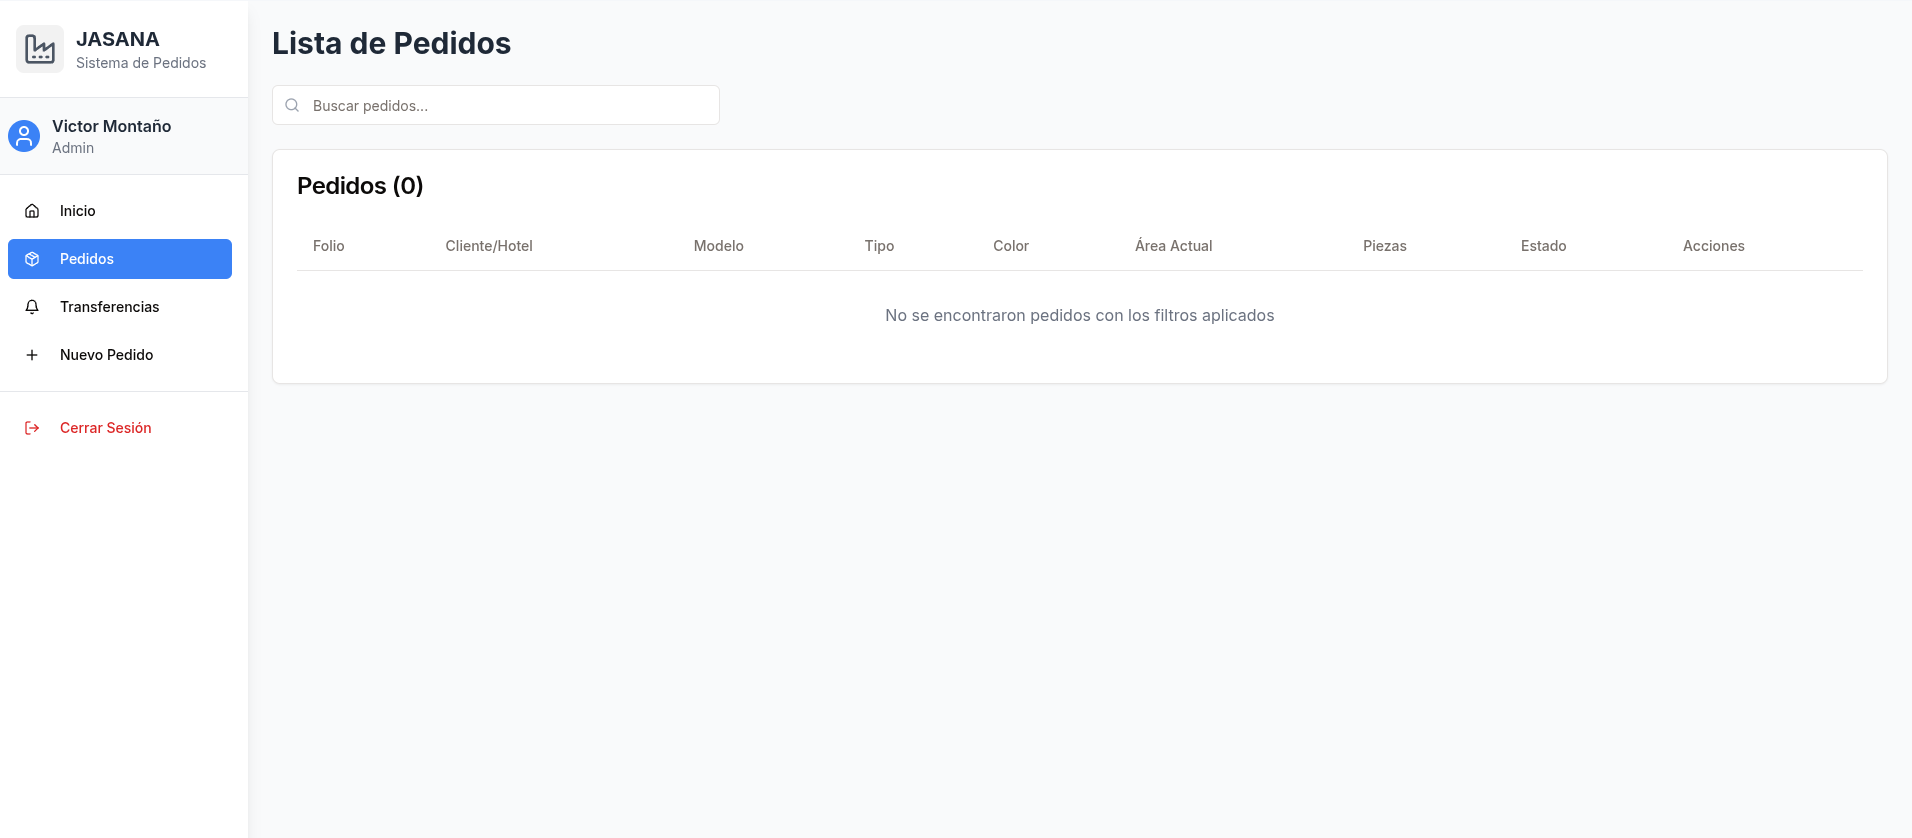
\includegraphics[width=0.9\textwidth]{V1.0.png}
    \caption{Versión 1.0 de la interfaz principal.}
    \label{fig:v1}
\end{figure}

\subsubsection{Versión 2.0: Refinamiento de la Navegación}
En la segunda iteración (Figura \ref{fig:v2}), se refinó la barra de navegación lateral, agrupando las opciones de manera más lógica (`Inicio`, `Pedidos`, `Reposiciones`) y añadiendo un botón de "Nuevo Pedido" para agilizar el flujo de trabajo del usuario. El título se actualizó a "Sistema de Pedidos" para ser más descriptivo.

\begin{figure}[H]
    \centering
    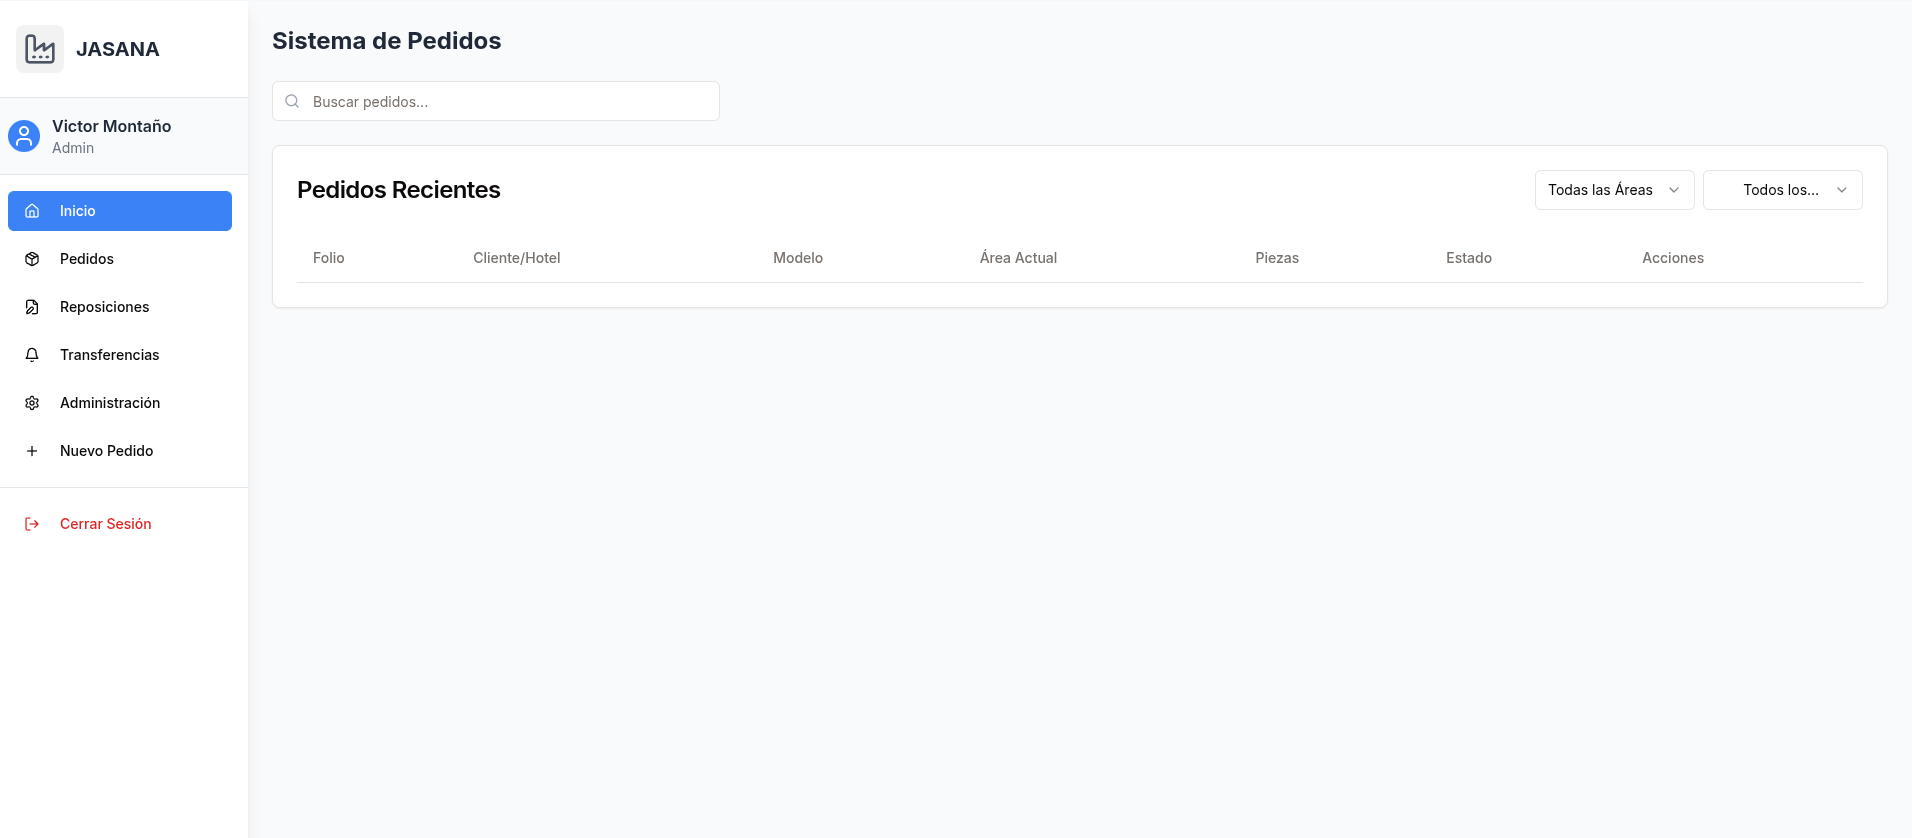
\includegraphics[width=0.9\textwidth]{V2.0.png}
    \caption{Versión 2.0 con mejoras en la navegación.}
    \label{fig:v2}
\end{figure}

\subsubsection{Versión 3.0: Enfoque Gerencial}
La versión 3.0 (Figura \ref{fig:v3}) representó un cambio de enfoque hacia una herramienta más gerencial, renombrando la aplicación a Centro de Control Empresarial. Se añadieron nuevas secciones en el menú como Reportes e Historial, anticipando la necesidad de funcionalidades de análisis y consulta.

\begin{figure}[H]
    \centering
    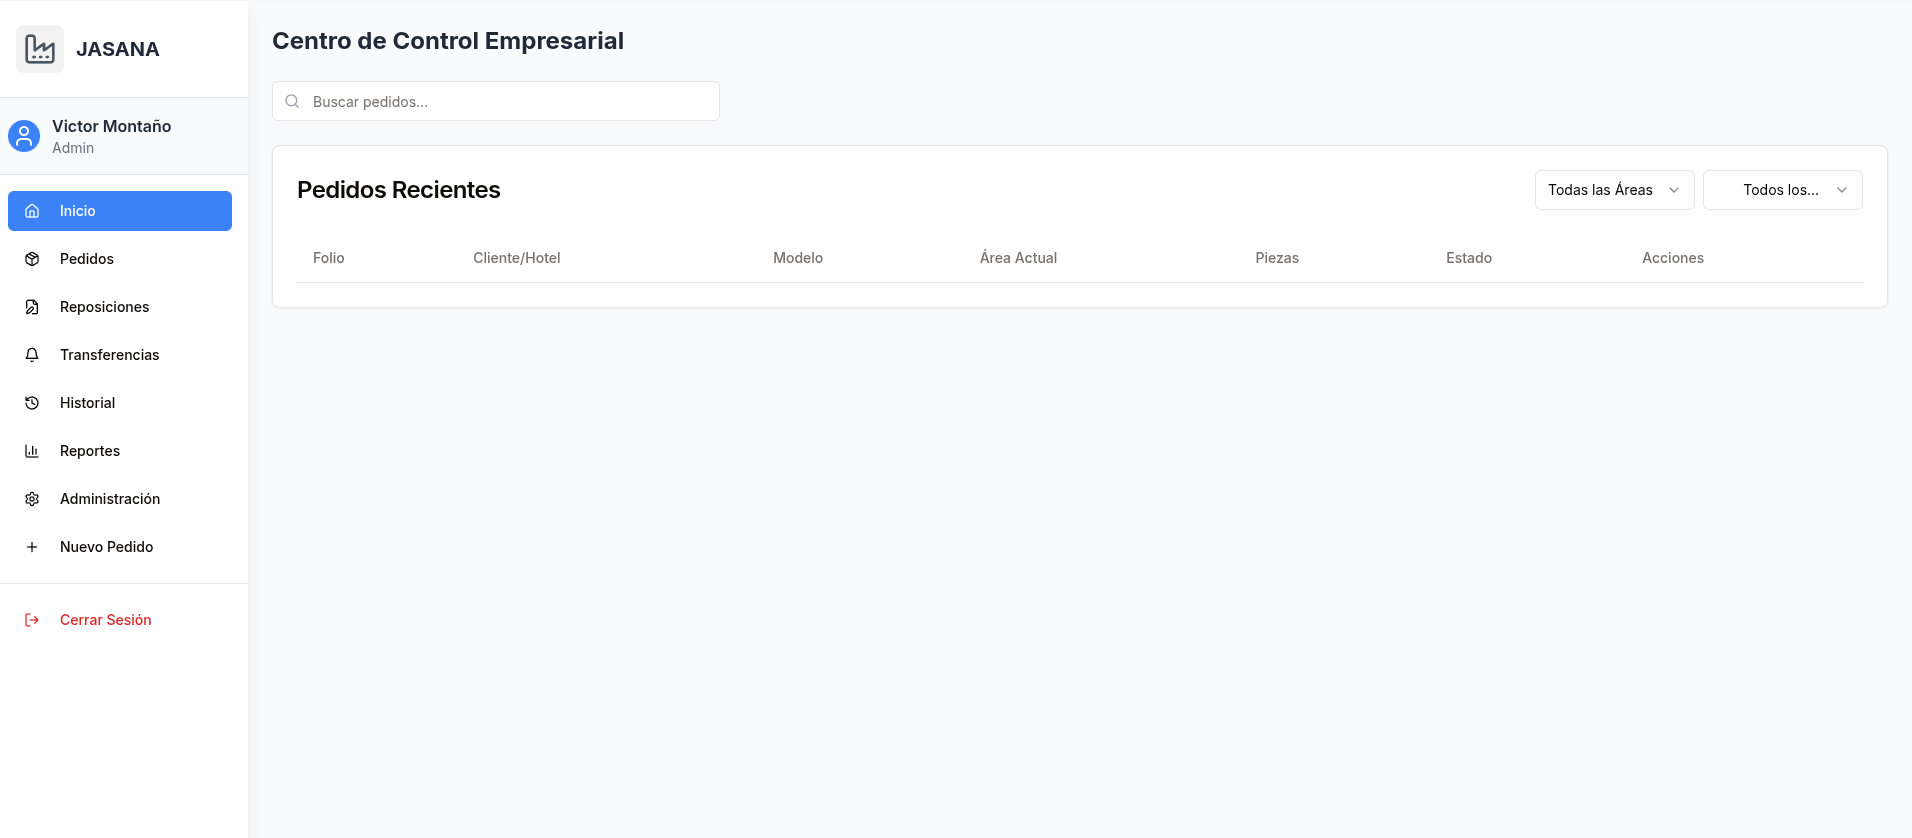
\includegraphics[width=0.9\textwidth]{V3.0.png}
    \caption{Versión 3.0 con enfoque en control y reportes.}
    \label{fig:v3}
\end{figure}

\subsubsection{Versión 4.0: Tablero de Control}
La versión final (Figura \ref{fig:v4}) consolida la evolución en un ''Tablero'' completo. La innovación principal es la adición de tarjetas de indicadores clave de rendimiento en la parte superior para una visualización rápida del estado del sistema ("Pedidos Activos", "Finalizados Hoy", etc.). Además, la sección de actividad reciente ahora diferencia entre "Pedidos" y "Reposiciones", ofreciendo una vista más granular. Este diseño final responde a la necesidad de tener tanto una vista operativa detallada como una vista gerencial resumida en una sola pantalla.

\begin{figure}[H]
    \centering
    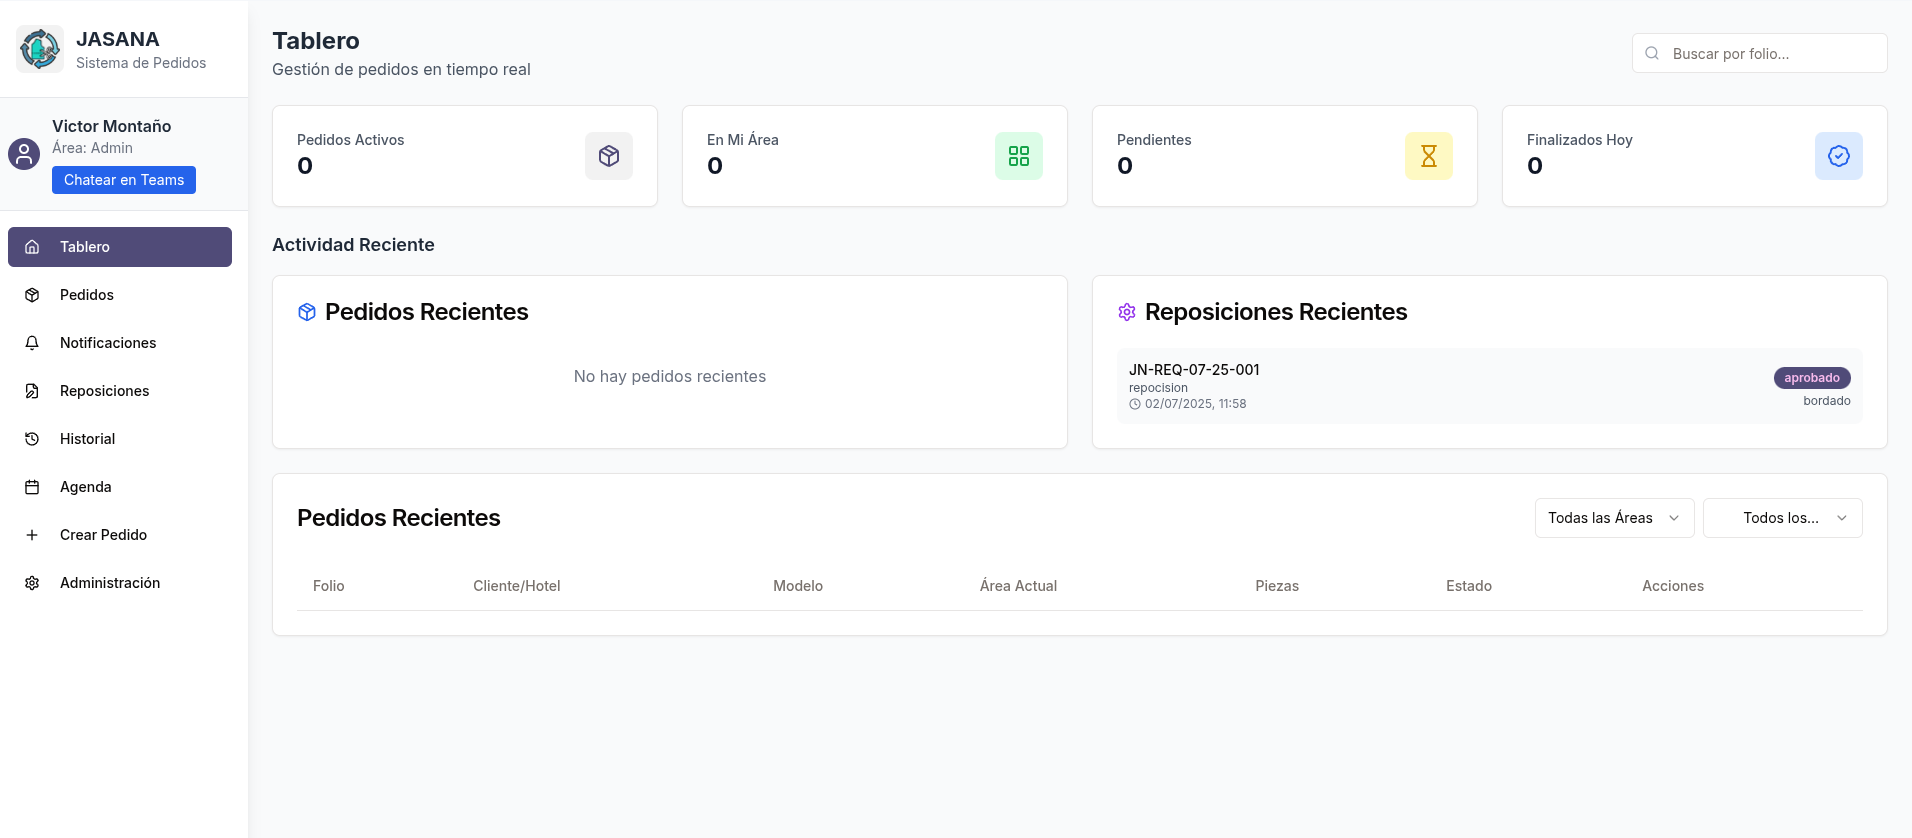
\includegraphics[width=0.9\textwidth]{V4.0.png}
    \caption{Versión final 4.0, implementada como un Tablero de Control y un logo añadido.}
    \label{fig:v4}
\end{figure}

Este proceso iterativo fue fundamental para refinar la aplicación.



\subsection{Entorno Gráfico Final}
\subsubsection{Vista Administrador: Panel de Reposiciones}
En la siguiente imagen (Figura \ref{fig:adminscreen}) podemos observar logeados desde el usuario de Administrador, todas las reposiciones que hay en curso, así como las ya completadas y las rechazadas por motivos de inconsistencia en los datos colocados en el form.

\begin{figure}[H]
    \centering
    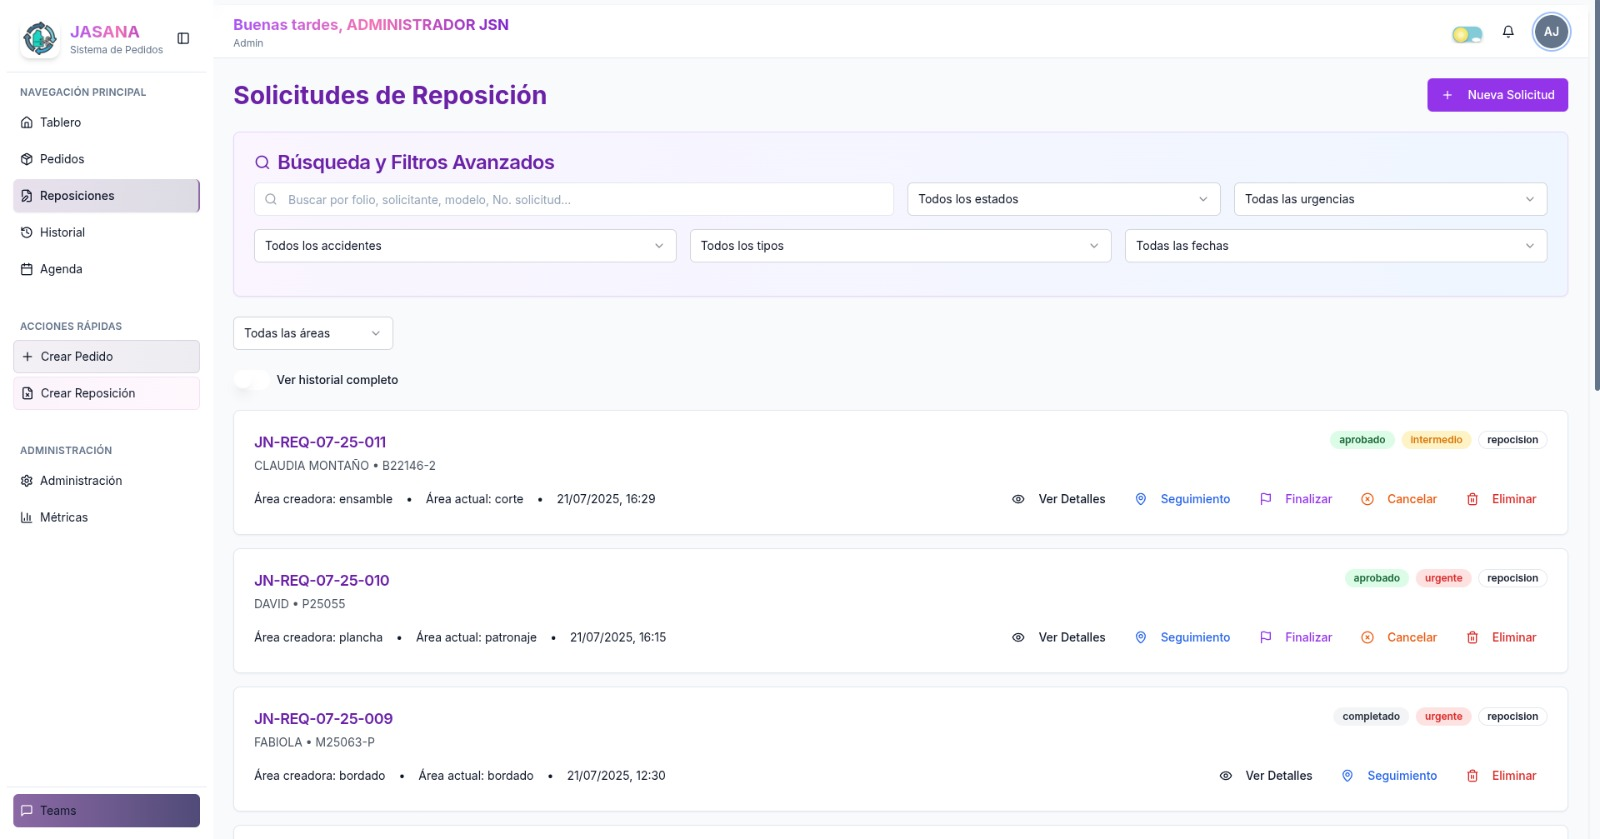
\includegraphics[width=0.9\textwidth]{pantalla_admin.jpg}
    \caption{Panel de control de las solicitudes de reposiciones o reprocesos.}
    \label{fig:adminscreen}
\end{figure}

\subsubsection{Vista Administrador: Manejo de usuarios}
Continuando con el usuario de administrador, en la siguiente imagen (Figura \ref{fig:usersadminscreen}) podemos observar una lista de todos los usuarios que estan registrados al sistema y al area que pertenecen, desde aquí le dimos la posibilidad de restablecer la contraseña de los usuarios, actualizar nombre de la persona, nombre de usuario o area en la que estan registrados, así cómo la posibilidad de crear nuevos usuarios o eliminar uno ya existente.

\begin{figure}[H]
    \centering
    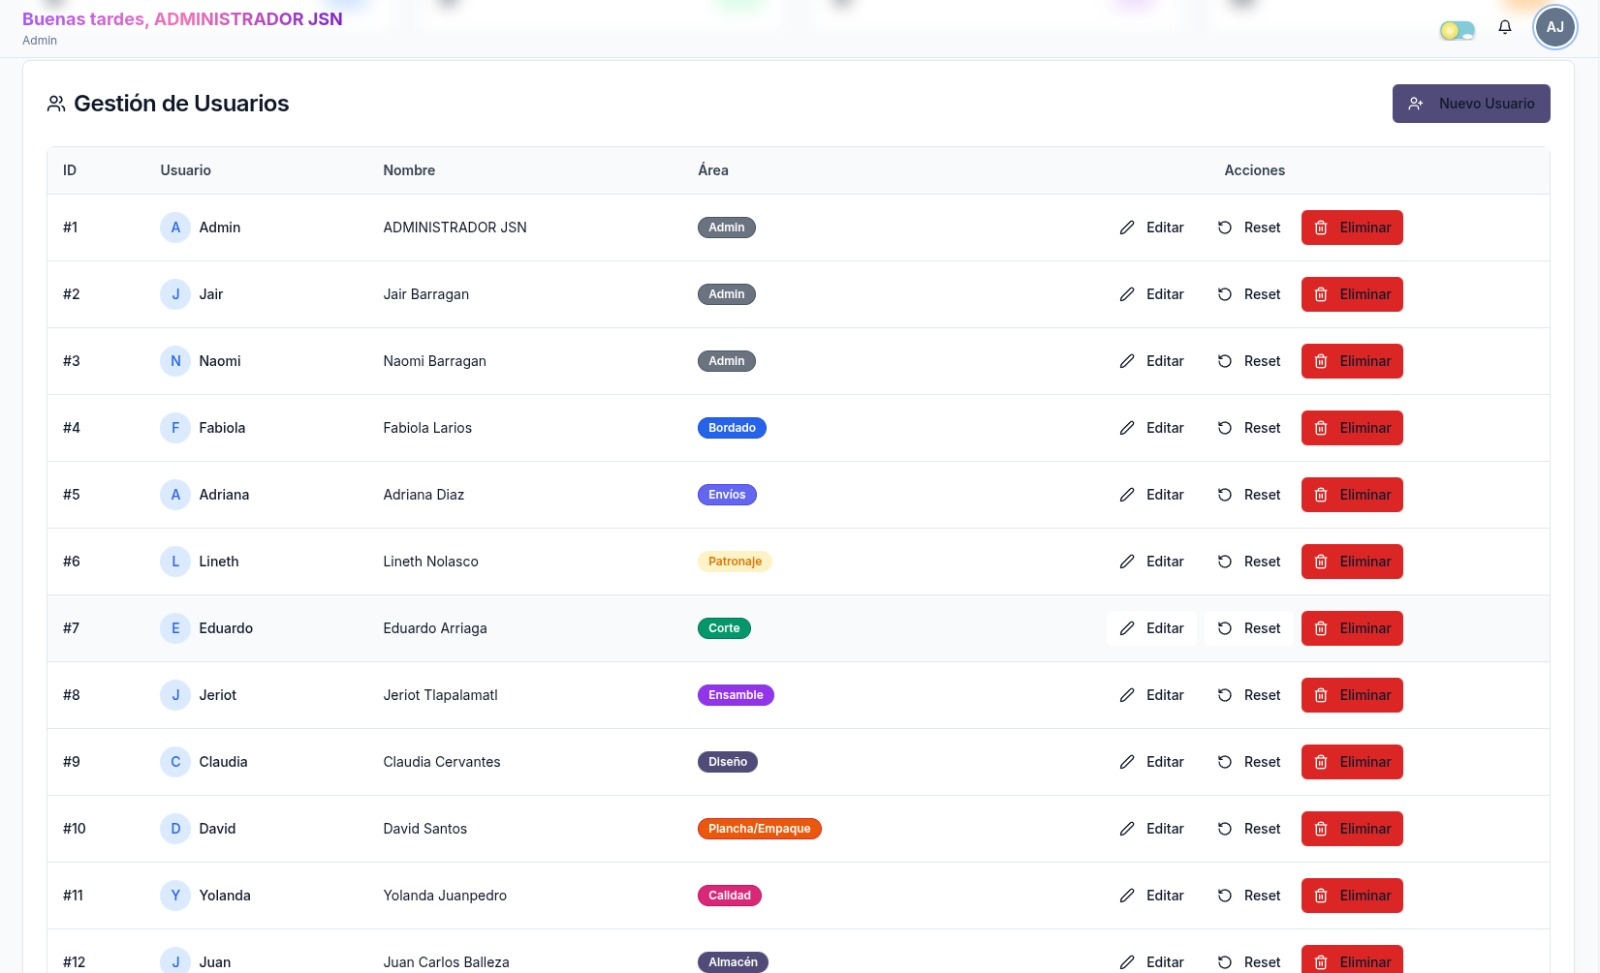
\includegraphics[width=0.9\textwidth]{admin_usuarios.jpg}
    \caption{Panel de control de usuarios registrados.}
    \label{fig:usersadminscreen}
\end{figure}

\subsubsection{Vista Administrador: Panel de control general}
En la siguiente imagen (Figura \ref{fig:adminpanel}) se observa una serie de opciones que solo usuarios registrados como admin pueden realizar, que va desde hacer copia de los usuarios dados de alta, así mismo como respaldarlos.
Se puede hacer una prueba de las notificaciones en dado caso de que lleguen a presentar una falla.
Tambien encontramos la opción de exportar reportes de manera general.
Y una opción para restablecer todo el sistema, dejando en blanco los datos, añadiendo una opcion para conservar  usuarios o no y restablecer los ids de usuario. Ver en imagen (Figura \ref{fig:borrartodo}).   .

\begin{figure}[H]
    \centering
    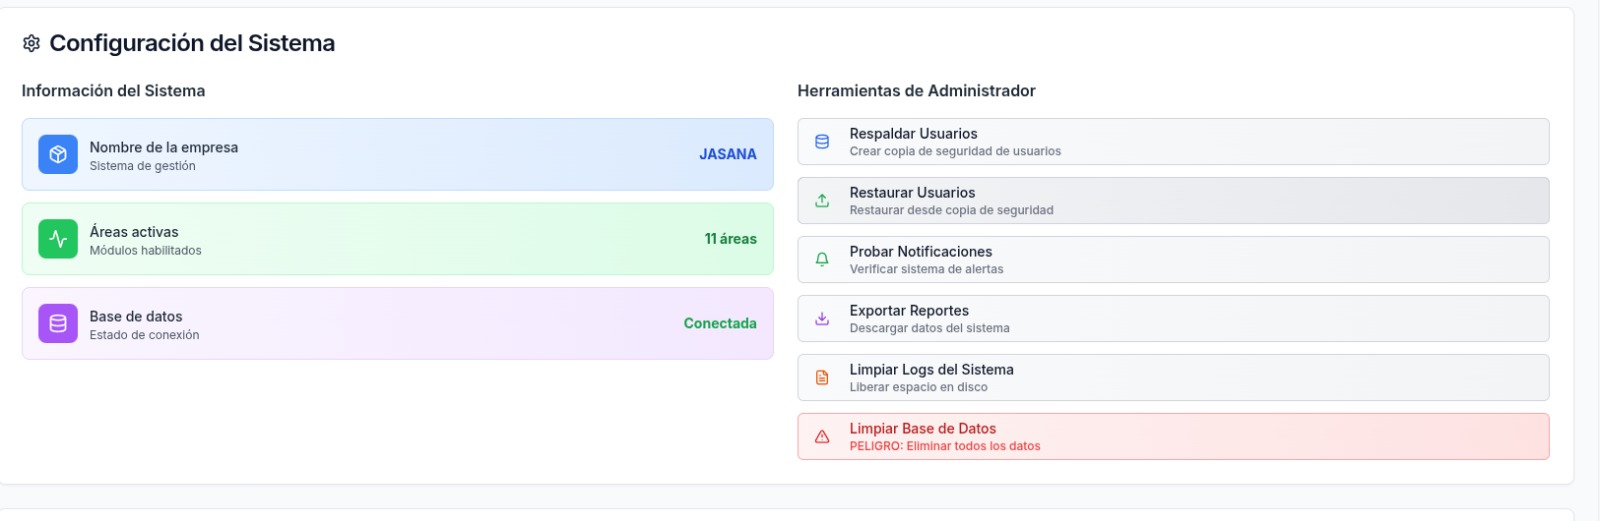
\includegraphics[width=0.9\textwidth]{admin_panel.jpg}
    \caption{Panel de control del sistema.}
    \label{fig:adminpanel}
\end{figure}
\begin{figure}[H]
    \centering
    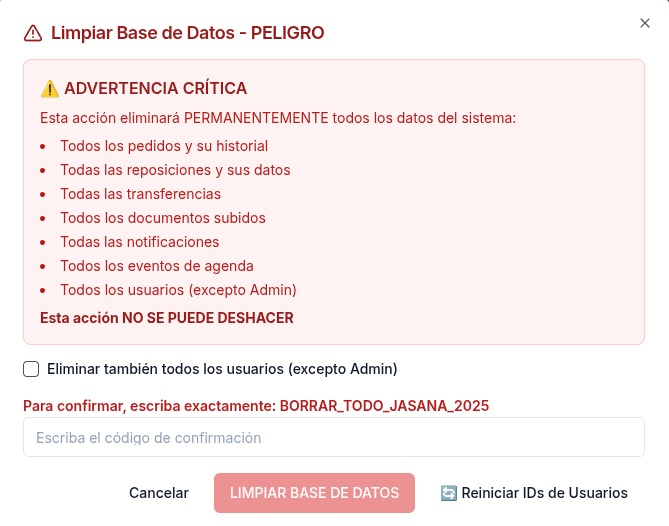
\includegraphics[width=0.9\textwidth]{limpi_bd.jpg}
    \caption{Confirmación para limpiar los datos del sistema.}
    \label{fig:borrartodo}
\end{figure}

\subsubsection{Vista General (todos los usuarios): Crear solicitud de reposición o reproceso}
A continuación se muestra en las imagenes (Figura \ref{fig:form1}) y (Figura \ref{fig:form2}) el formulario que es necesario para generar una solicitud, los datos que se piden fueron tomados de un formato ya existente en la empresa, esto para facilitar la familiarización de los usuarios.

\begin{figure}[H]
    \centering
    
\includegraphics[width=0.9\textwidth]{form_repo1.jpg}
    \caption{Primera parte del formulario de solicitudes.}
    \label{fig:form1}
\end{figure}
\begin{figure}[H]
    \centering
    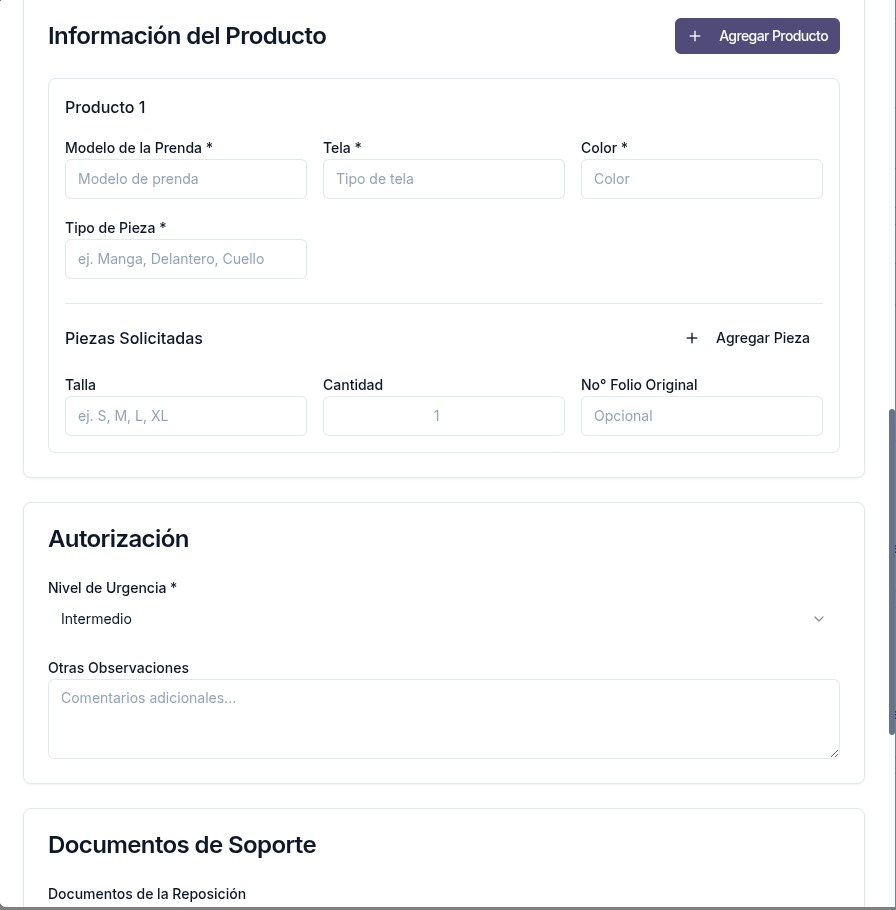
\includegraphics[width=0.9\textwidth]{form_repo2.jpg}
    \caption{Segunda parte del formulario de solicitudes.}
    \label{fig:form2}
\end{figure}
\subsubsection{Métricas (solo admins): Ver reportes de daños}
A continuación se muestra en las imagenes (Figura \ref{fig:metricas1}), (Figura \ref{fig:metricas2}) y (Figura \ref{fig:metricas3}) el apartado de métricas, que sirve para darle una idea al usuario de que areas son las más problematicas, que pedidos tienen meayor solicitudes de reposición o reprocesos y que causas de daños son las más cómunes, se le dio la opción de bajar sus reportes como formato .xlxs.

\begin{figure}[H]
    \centering
    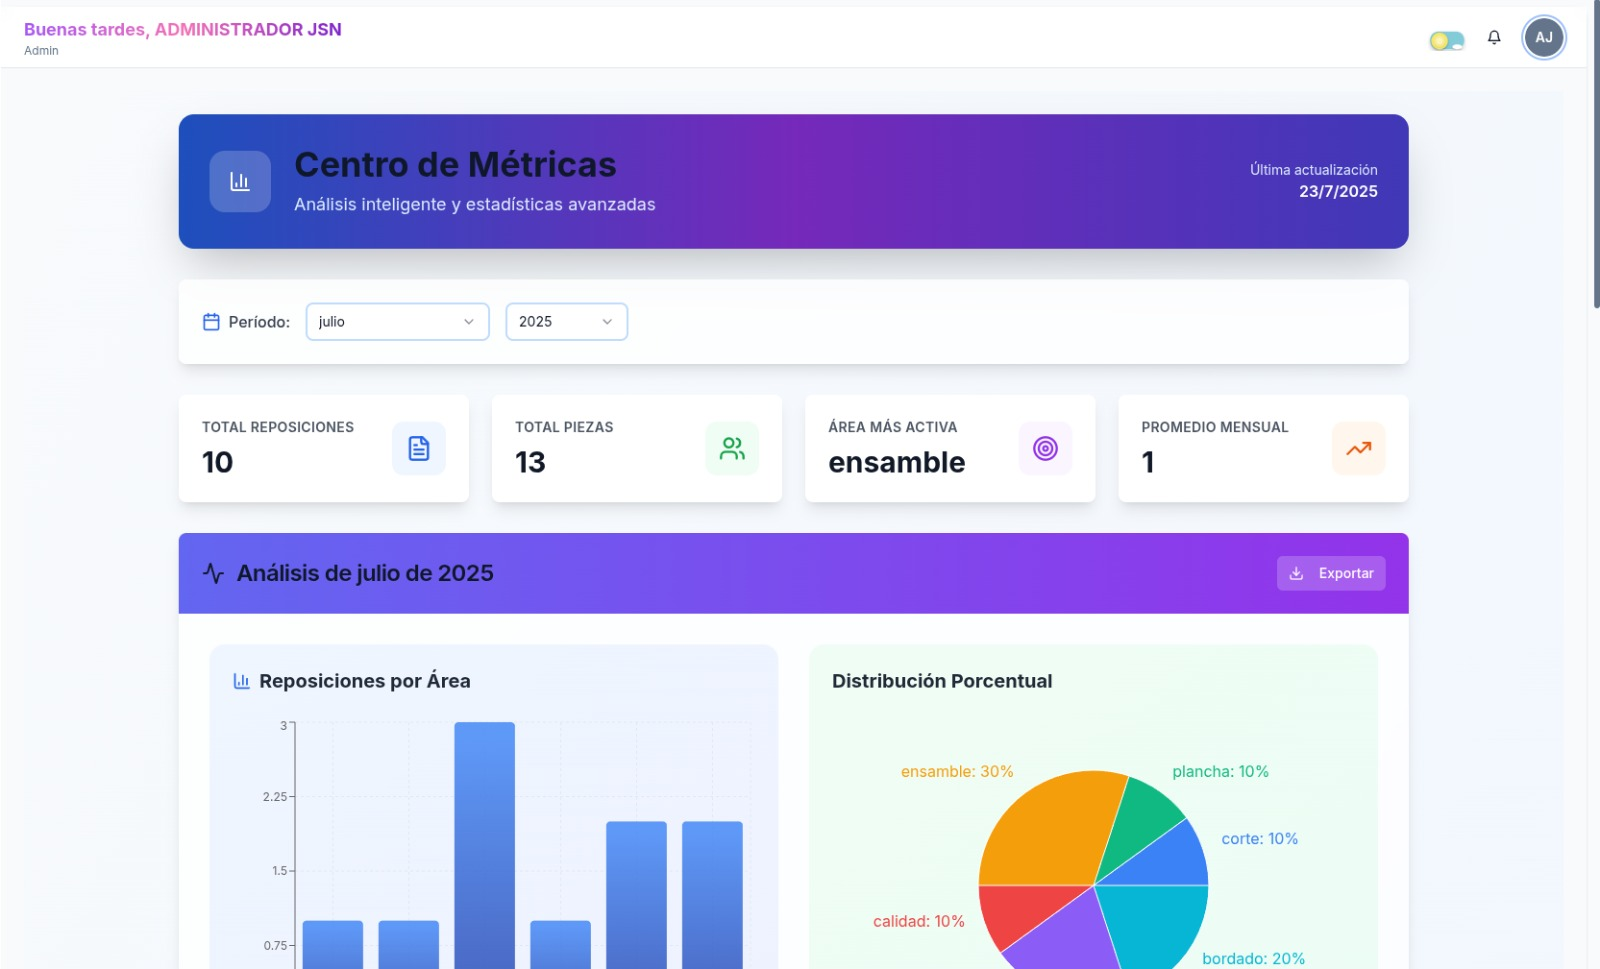
\includegraphics[width=0.9\textwidth]{metricas1.jpg}
    \caption{Parte 1 del apartado de Métricas.}
    \label{fig:metricas1}
\end{figure}
\begin{figure}[H]
    \centering
    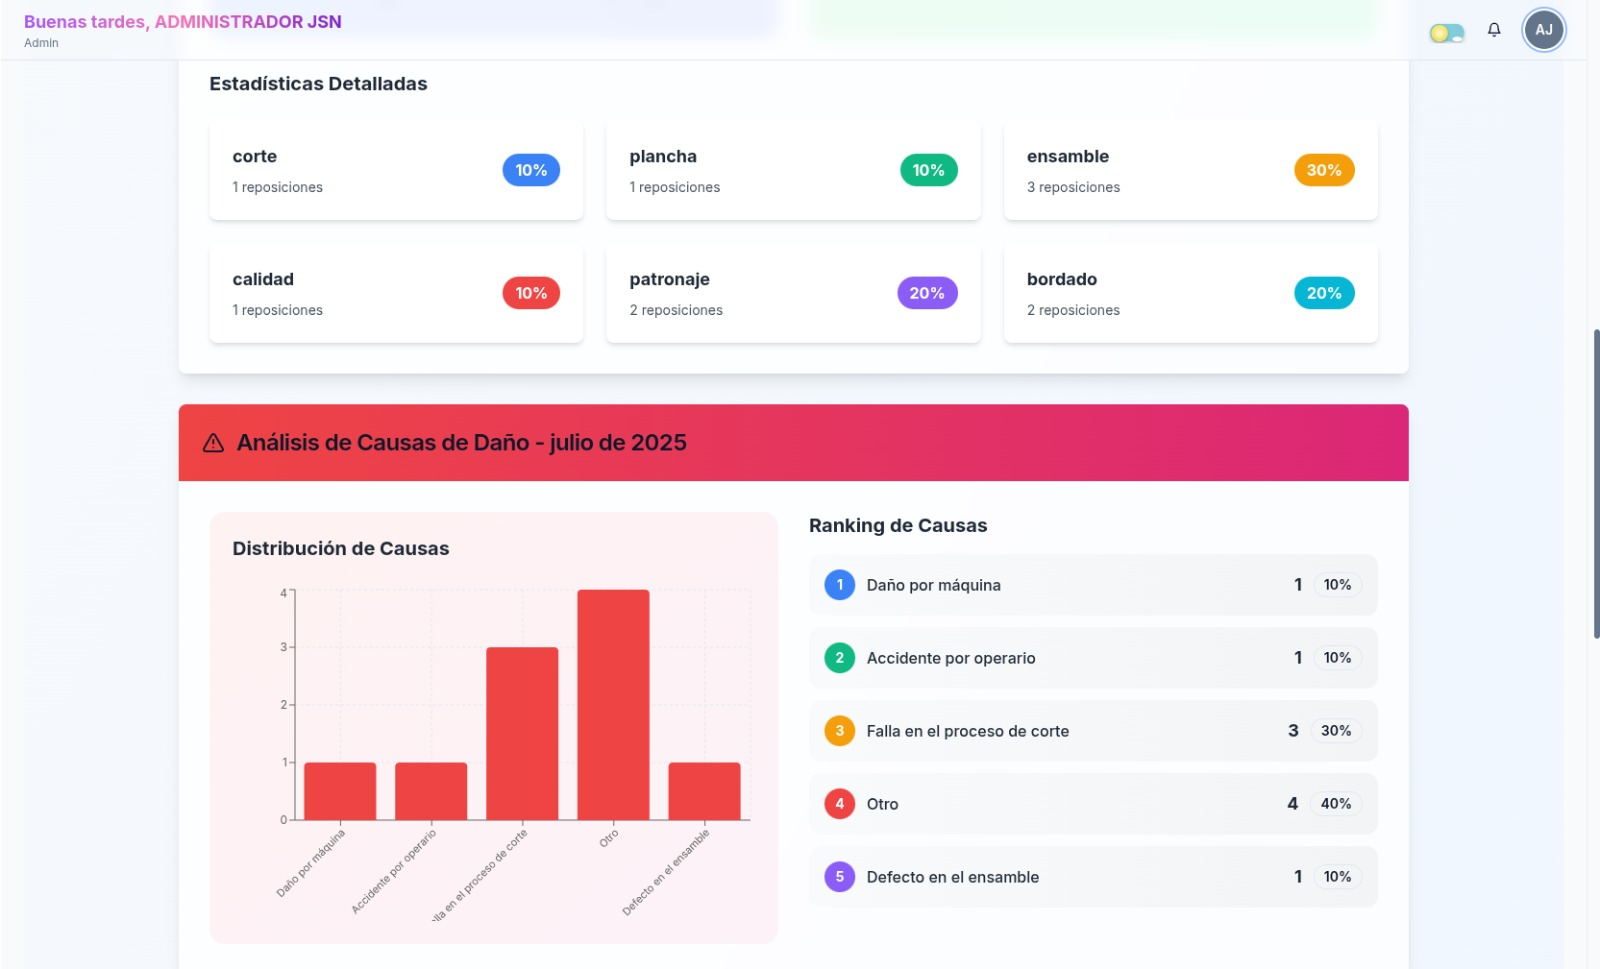
\includegraphics[width=0.9\textwidth]{metricas2.jpg}
    \caption{Parte 2 del apartado de Métricas.}
    \label{fig:metricas2}
\end{figure}
\begin{figure}[H]
    \centering
    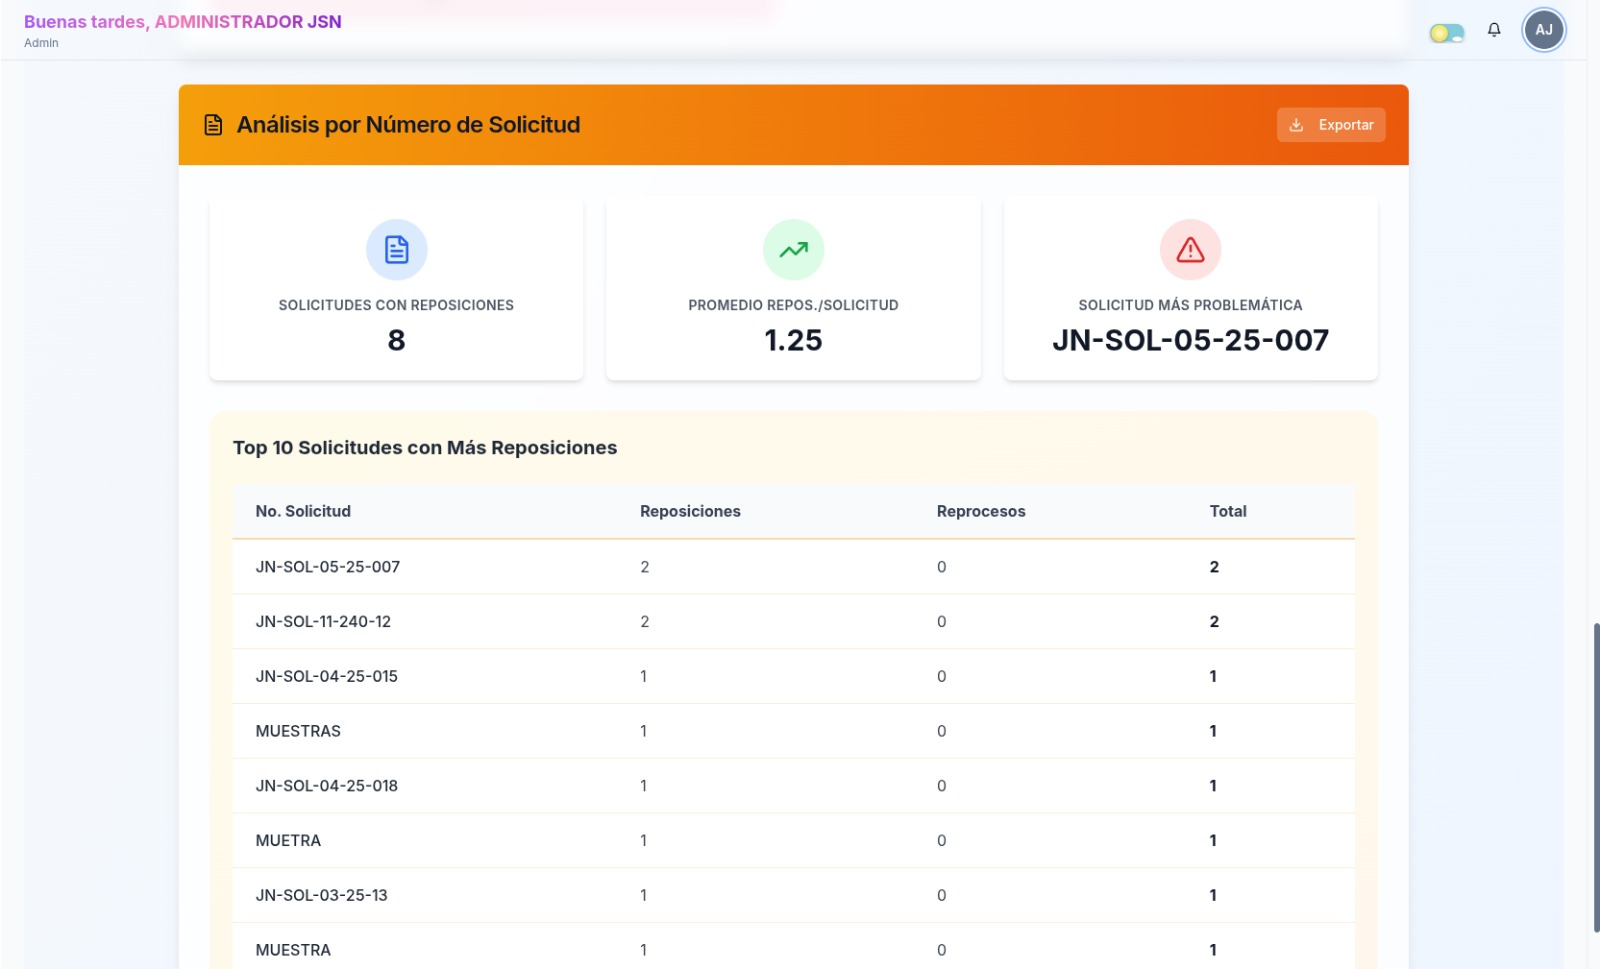
\includegraphics[width=0.9\textwidth]{metricas3.jpg}
    \caption{Parte 3 del apartado de Métricas.}
    \label{fig:metricas3}
\end{figure}

\subsubsection{Detalles de las solicitudes (todos los usuarios)}
A continuación se muestra en las imagenes (Figura \ref{fig:detalles1}) y (Figura \ref{fig:detalles2}) estos son los detalles de la solicitud generada, esto permite obtener una información previa a aceptar la transferencia de la reposición de un área a otra, también sirve para determinar si se aprueba o rechaza una solicitud.

\begin{figure}[H]
    \centering
    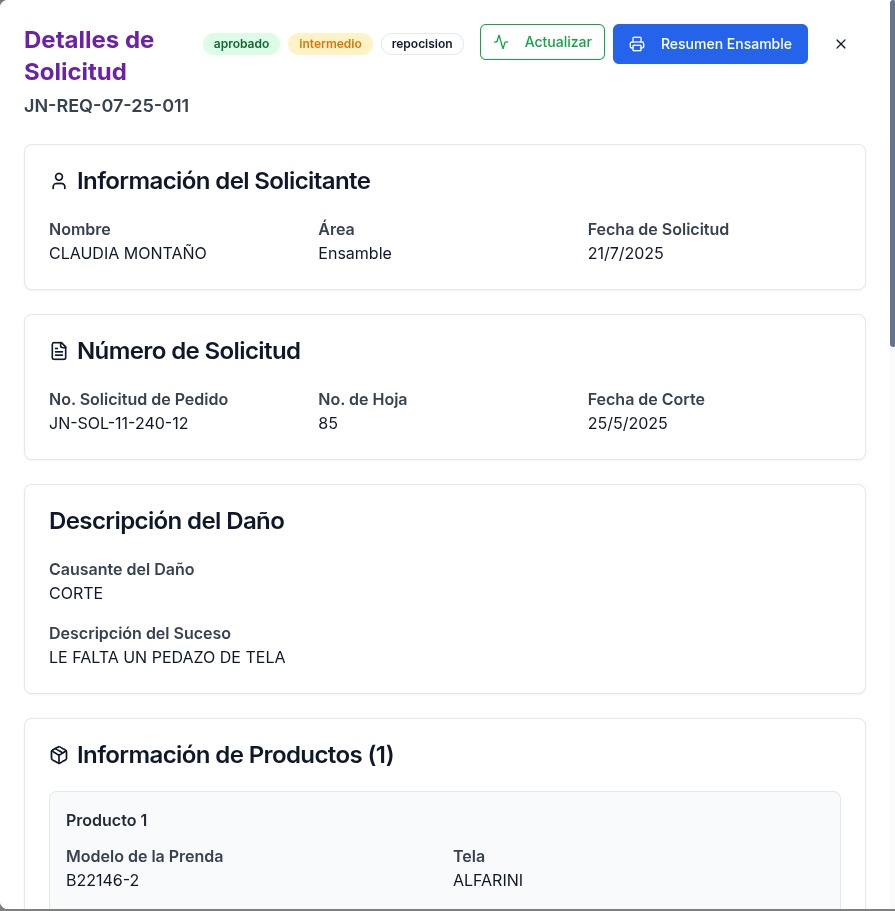
\includegraphics[width=0.9\textwidth]{detalles_rep1.jpg}
    \caption{Parte 1 de los detalles de la solicitud.}
    \label{fig:detalles1}
\end{figure}

\begin{figure}[H]
    \centering
    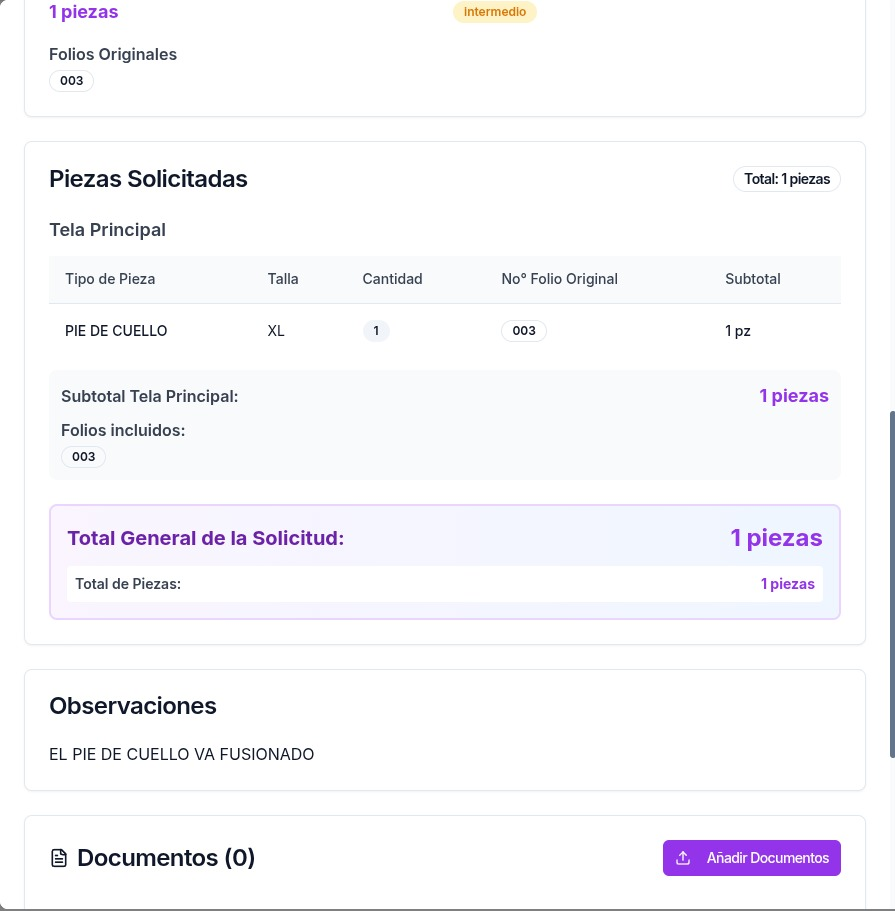
\includegraphics[width=0.9\textwidth]{detalles_rep2.jpg}
    \caption{Parte 2 de los detalles de la solicitud.}
    \label{fig:detalles2}
\end{figure}
 \textbf{Notificaciones:}
 Cuando una solicitud se genera, los Admins o el area de Envios puede determinar la acción que se tomará, en las siguientes imagenes(Figura \ref{noti1} a \ref{notifinal}) se describe con más detalle el funcionamiento y vistas de las notificaciones.
 \begin{figure}
   \centering
   
\includegraphics[width=0.9\textwidth]{noti1.jpg}
   \caption{Notificación desde vista de admin}\label{noti1}
 \end{figure}

 \begin{figure}
   \centering
   
\includegraphics[width=0.9\textwidth]{admvista.jpg}
   \caption{Solicitud desde vista de admin, muestra las acciones a realizar}\label{admvista}
 \end{figure}

 \begin{figure}
   \centering
   
\includegraphics[width=0.9\textwidth]{notiaprov.jpg}
   \caption{Notificación de solicitud aprobada}\label{notiaprov}
 \end{figure}

 \begin{figure}
   \centering
   
\includegraphics[width=0.9\textwidth]{vistarecep.jpg}
   \caption{Vista de la solicitud en el área receptora}\label{vistarecep}
 \end{figure}

 \begin{figure}
   \centering
   
\includegraphics[width=0.9\textwidth]{historial.jpg}
   \caption{Historial de las solicitudes de transferencia y su estatus}\label{historial}
 \end{figure}

 \begin{figure}
   \centering
   
\includegraphics[width=0.9\textwidth]{tiempo.jpg}
   \caption{Vista del registro del tiempo (ingresado anteriormente)}\label{tiempo}
   \end{figure}
   
    \begin{figure}
   \centering
   
\includegraphics[width=0.9\textwidth]{notifinal.jpg}
   \caption{Una vez culminado el proceso de reposición, el area creadora tiene la opcion de pedir la finalización de dicha solicitud, misma que se les notificara a las areas de Admin y Envíos para poder finalizarla}\label{notifinal}
   \end{figure}
    


\section{Pruebas}

\subsection{Plan de pruebas}
El objetivo de este plan es validar el correcto funcionamiento del Sistema de Gesti\'on de Reprocesos y Pedidos desarrollado para Corporativo Textil JSN. Se busca garantizar que cada funcionalidad implementada cumpla con los requerimientos definidos y que el sistema opere de forma estable bajo condiciones normales.

\subsection{Alcance de las Pruebas}
Este plan contempla pruebas manuales enfocadas en la validaci\'on funcional y no funcional de los m\'odulos principales del sistema:

\begin{itemize}
    \item Registro de solicitudes
    \item Registro y gesti\'on de piezas
    \item Aprobaci\'on y rechazo de solicitudes
    \item Registro de avance de reproceso
    \item Autenticaci\'on y control de permisos
\end{itemize}


\subsection{Criterios de Entrada y Salida}
\begin{itemize}
    \item \textbf{Criterios de entrada:}
    \begin{itemize}
        \item Sistema desplegado correctamente en entorno de pruebas
        \item Base de datos operativa con datos de ejemplo
        \item Navegador actualizado y acceso de usuario autenticado
    \end{itemize}

    \item \textbf{Criterios de salida:}
    \begin{itemize}
        \item Todos los casos de prueba ejecutados
        \item Al menos el 90\% de los casos exitosos
        \item Documentaci\'on de incidencias o errores detectados
    \end{itemize}
\end{itemize}

\subsection{Entorno de Pruebas}
\begin{itemize}
    \item Navegador: Mozilla Firefox / Google Chrome / Microsoft Edge / Opera GX / Brave
    \item Sistema Operativo: Linux Mint 21.3 Cinnamon 6
    \item Backend: Node.js 20.10 
    \item Frontend: React 18.2  
    \item Base de Datos: PostgreSQL 16
\end{itemize}

%\subsection{Casos de Prueba}
%\begin{table}[H]
%\centering
%\begin{tabular}{|c|p{4.5cm}|p{3.5cm}|p{3.5cm}|c|}
%\hline
%\textbf{ID} & \textbf{Descripción} & \textbf{Entrada} & \textbf{Resultado Esperado} & \textbf{Estado} \\
%\hline
%PF-Lo001 & Login con credenciales v\'alidas & Usuario: supervisor@jsn.mx, Contrase\~na: segura123 & Acceso exitoso al dashboard & Correcto \\
%\hline
%PF-SO001 & Registro de solicitud nueva & Formulario completo con datos v\'alidos & Solicitud registrada y folio generado & Correcto \\
%\hline
%PF-PZ001 & Registro de varias piezas en solicitud & 3 piezas con datos correctos & Piezas guardadas asociadas al folio & Correcto \\
%\hline
%PF-SU001 & Aprobaci\'on de solicitud por supervisor & Estado en revisi\'on + acci\'on aprobar & Cambio de estado a \"Aprobada\" & Correcto \\
%\hline
%PF-AV001 & Registro de avance de reproceso & Horas de inicio/fin + operador + \'area & Registro de etapa completado & Correcto \\
%\hline
%PF-FI001 & Finalizaci\'on del proceso & Todas las etapas finalizadas & Estado de solicitud \"Completado\" + notificaciones & Correcto \\
%\hline
%\end{tabular}
%\caption{Casos de prueba funcionales del sistema}
%\end{table}









\subsection{Casos de prueba}
Como parte fundamental del proceso final del desarrollo de esta aplicación, se plantearon diferentes tipos de pruebas para corroborar la funcionalidad, fluidez, y calidad general del sistema, sobre los resultados arrojados por estas mismas se decidió reajustar y realizar correcciones y posibles mejoras para una implementación que cumpla con los requerimientos previamente levantados y así entregar un resultado con la mayor calidad posible.
En las próximas imágenes (Figura \ref{Lo001} a \ref{Pe007}) se puede encontrar con más detalle cada caso de prueba ejecutado junto a sus resultados y acciones tomadas, además y como pequeño detalle, cada Id lleva un distintivo que refiere al tipo de prueba realizada, p. ejemplo PF-Lo001 es Prueba Funcional de Login 001.


\newpage

\begin{figure}[H]
  \centering
  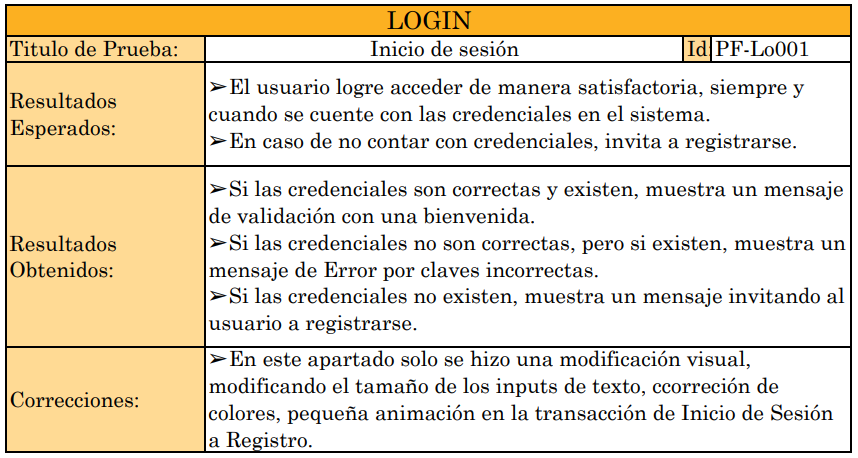
\includegraphics[width=0.9\textwidth]{PF-Lo001.png}
  \caption{Caso de Pruebas Login 001}\label{Lo001}
\end{figure}

\begin{figure}[H]
  \centering
  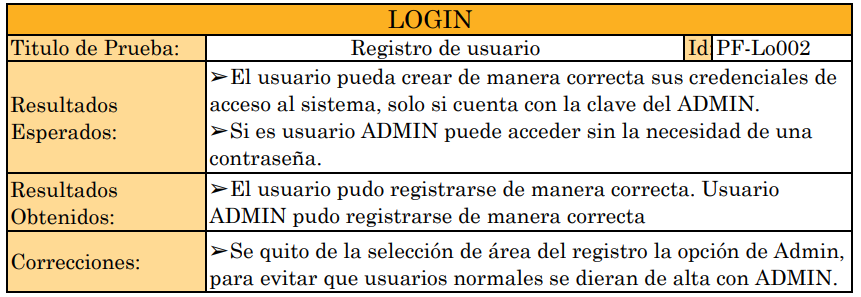
\includegraphics[width=0.9\textwidth]{PF-Lo002.png}
  \caption{Caso de Pruebas Login 002}\label{Lo002}
\end{figure}


\begin{figure}[H]
  \centering
  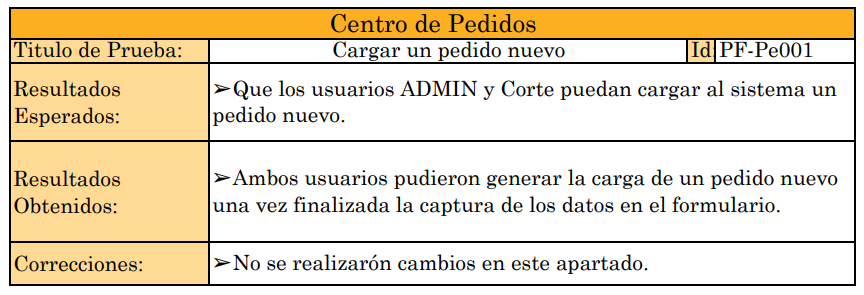
\includegraphics[width=0.9\textwidth]{PF-Pe001.png}
  \caption{Caso de Pruebas Centro de Pedidos 001}\label{Pe001}
\end{figure}

\begin{figure}[H]
  \centering
  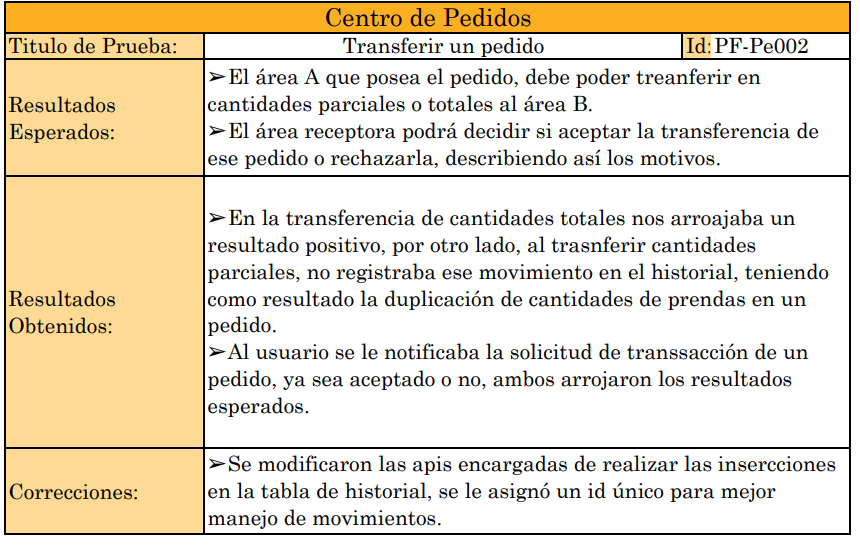
\includegraphics[width=0.9\textwidth]{PF-Pe002.png}
  \caption{Caso de Pruebas Centro de Pedidos 002}\label{Pe002}
\end{figure}

\begin{figure}[H]
  \centering
  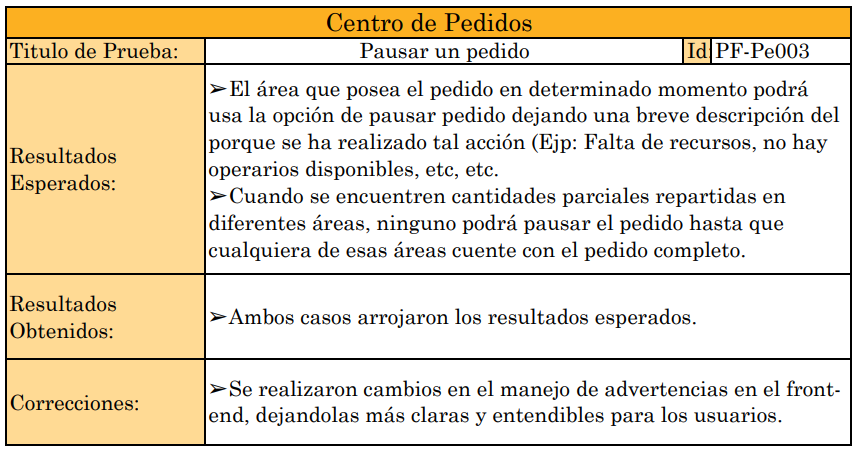
\includegraphics[width=0.9\textwidth]{PF-Pe003.png}
  \caption{Caso de Pruebas Centro de Pedidos 003}\label{Pe003}
\end{figure}


\begin{figure}[H]
  \centering
  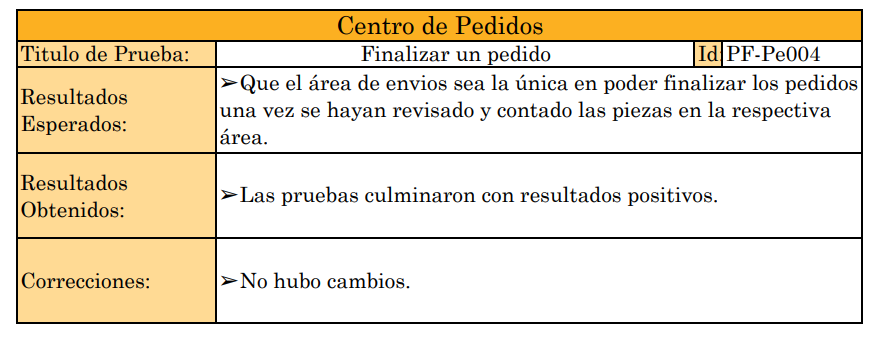
\includegraphics[width=0.9\textwidth]{PF-Pe004.png}
  \caption{Caso de Pruebas Centro de Pedidos 004}\label{Pe004}
\end{figure}


\begin{figure}[H]
  \centering
  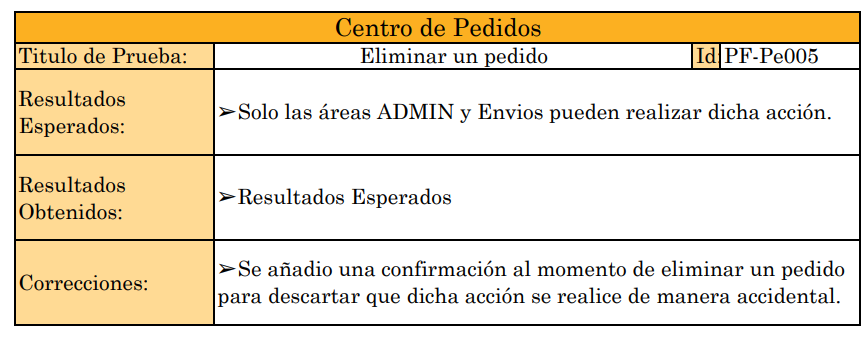
\includegraphics[width=0.9\textwidth]{PF-Pe005.png}
  \caption{Caso de Pruebas Centro de Pedidos 05}\label{Pe005}
\end{figure}

\begin{figure}[H]
  \centering
  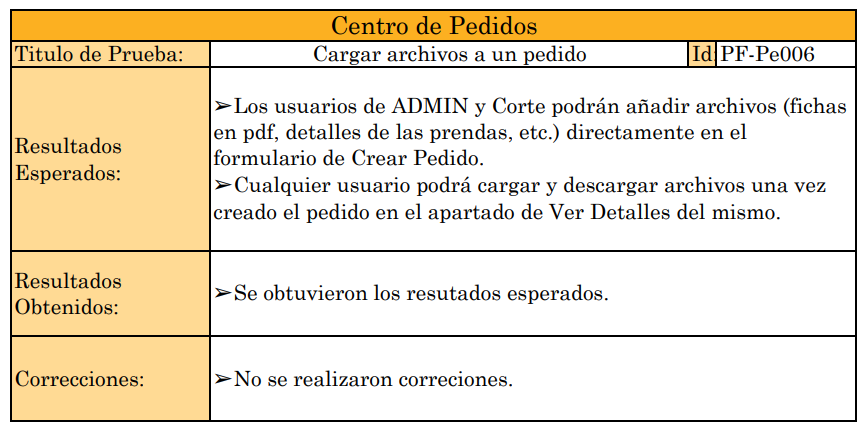
\includegraphics[width=0.9\textwidth]{PF-Pe006.png}
  \caption{Caso de Pruebas Centro de Pedidos 006}\label{Pe006}
\end{figure}


\begin{figure}[H]
  \centering
  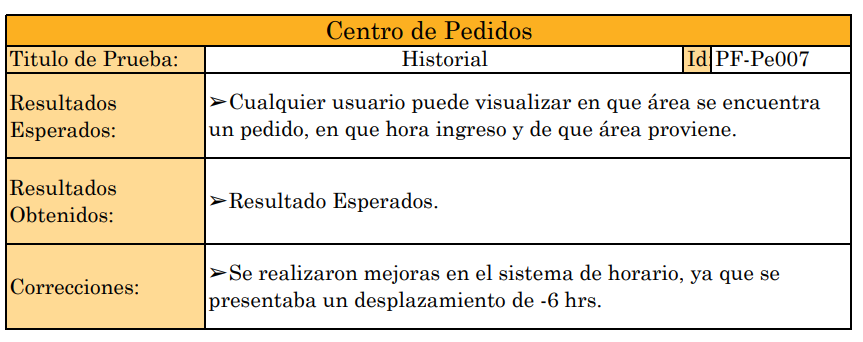
\includegraphics[width=0.9\textwidth]{PF-Pe007.png}
  \caption{Caso de Pruebas Centro de Pedidos 007}\label{Pe007}
\end{figure}

\begin{figure}[H]
  \centering
  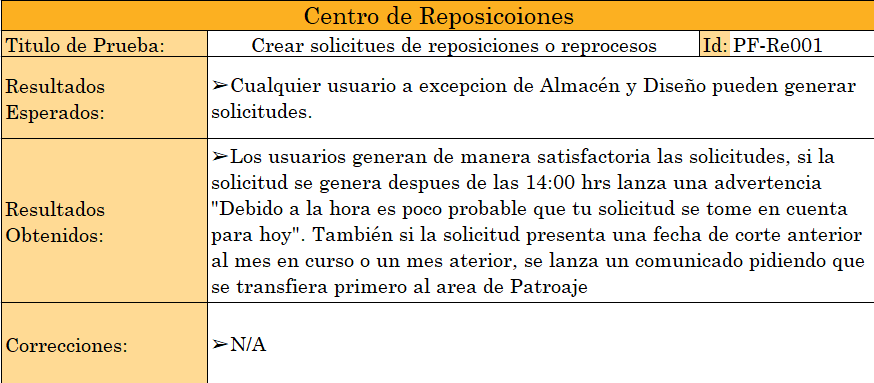
\includegraphics[width=0.9\textwidth]{Rep_01.png}
  \caption{Caso de Pruebas Centro de Reposiciones 001}\label{Re001}
\end{figure}

\begin{figure}[H]
  \centering
  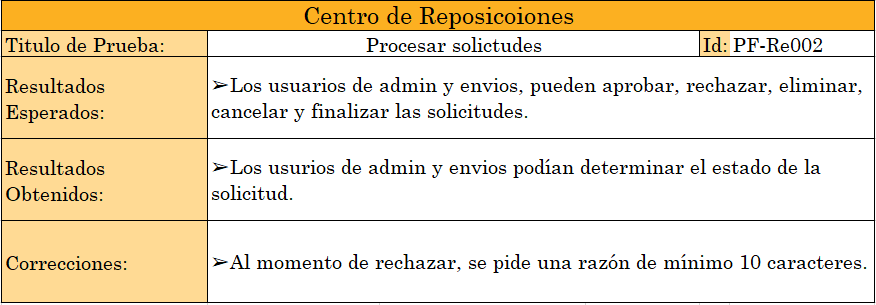
\includegraphics[width=0.9\textwidth]{Rep_02.png}
  \caption{Caso de Pruebas Centro de Reposiciones 002}\label{Re002}
\end{figure}

\begin{figure}[H]
  \centering
  \includegraphics[width=0.9\textwidth]{Rep_03.png}
  \caption{Caso de Pruebas Centro de Reposiciones 003}\label{Pe003}
\end{figure}

\begin{figure}[H]
  \centering
  \includegraphics[width=0.9\textwidth]{Rep_04.png}
  \caption{Caso de Pruebas Centro de Reposiciones 004}\label{Pe004}
\end{figure}


\begin{figure}[H]
  \centering
  \includegraphics[width=0.9\textwidth]{Admi_01.png}
  \caption{Caso de Pruebas Centro de Administración 001}\label{Adm001}
\end{figure}


\subsection{Resultados}
Todos los casos de prueba definidos fueron ejecutados exitosamente durante la fase de validaci\'on. Las funcionalidades principales operan de acuerdo a lo especificado en los requerimientos, sin presentar errores fatales, además se aprovecharon areas de mejora que anteriormente no estaban bien definidas ni contempladas.




% CAPITULO RESULTADOS(estatus del proyecto y posibles mejoras) Y CONCLUSIONES(problemas presentados, costos, restrasos, cumplimiento de objetivos, etc)
%____________________________________________________________________________________________________________________


\chapter{Resultados y Conclusiones}
\newpage

\section{Resultados}

A continuación se presentan los resultados obtenidos de la encuesta de satisfacción aplicada a usuarios de distintas áreas de la aplicación web.

\subsection*{Área: Bordado}
\begin{itemize}
    \item \textbf{Diseño visual:} Bueno
    \item \textbf{Facilidad de uso:} Fácil
    \item \textbf{Intuitiva:} De acuerdo
    \item \textbf{Cambio en el trabajo:} Ha mejorado
    \item \textbf{Sugerencias:} Sería útil tener accesos rápidos a las órdenes más recientes y una alerta para cuando hay retrasos.
\end{itemize}

\subsection*{Área: Corte}
\begin{itemize}
    \item \textbf{Diseño visual:} Aceptable
    \item \textbf{Facilidad de uso:} Neutral
    \item \textbf{Intuitiva:} Neutral
    \item \textbf{Cambio en el trabajo:} Se mantiene igual
    \item \textbf{Sugerencias:} Mejorar el buscador, a veces no encuentra los productos por nombre.
\end{itemize}

\subsection*{Área: Diseño}
\begin{itemize}
    \item \textbf{Diseño visual:} Excelente
    \item \textbf{Facilidad de uso:} Muy fácil
    \item \textbf{Intuitiva:} Totalmente de acuerdo
    \item \textbf{Cambio en el trabajo:} Ha mejorado mucho
    \item \textbf{Sugerencias:} Muy contentos con la interfaz, solo añadir opción de ver cambios históricos.
\end{itemize}

\subsection*{Área: Patronaje}
\begin{itemize}
    \item \textbf{Diseño visual:} Bueno
    \item \textbf{Facilidad de uso:} Fácil
    \item \textbf{Intuitiva:} De acuerdo
    \item \textbf{Cambio en el trabajo:} Ha mejorado
    \item \textbf{Sugerencias:} A veces la carga de archivos es lenta, revisar tiempos o conexión.
\end{itemize}

\subsection*{Área: Plancha}
\begin{itemize}
    \item \textbf{Diseño visual:} Aceptable
    \item \textbf{Facilidad de uso:} Fácil
    \item \textbf{Intuitiva:} Neutral
    \item \textbf{Cambio en el trabajo:} Ha mejorado
    \item \textbf{Sugerencias:} Un pequeño tutorial ayudaría para nuevos usuarios.
\end{itemize}

\subsection*{Área: Envíos}
\begin{itemize}
    \item \textbf{Diseño visual:} Bueno
    \item \textbf{Facilidad de uso:} Fácil
    \item \textbf{Intuitiva:} De acuerdo
    \item \textbf{Cambio en el trabajo:} Ha mejorado
    \item \textbf{Sugerencias:} Agregar una vista rápida de pedidos pendientes por día.
\end{itemize}

\subsection*{Área: Calidad}
\begin{itemize}
    \item \textbf{Diseño visual:} Bueno
    \item \textbf{Facilidad de uso:} Fácil
    \item \textbf{Intuitiva:} De acuerdo
    \item \textbf{Cambio en el trabajo:} Ha mejorado mucho
    \item \textbf{Sugerencias:} Todo bien, pero podría destacar más los errores marcados por otras áreas.
\end{itemize}

\subsection*{Área: Almacén}
\begin{itemize}
    \item \textbf{Diseño visual:} Bueno
    \item \textbf{Facilidad de uso:} Fácil
    \item \textbf{Intuitiva:} De acuerdo
    \item \textbf{Cambio en el trabajo:} Ha mejorado
    \item \textbf{Sugerencias:} Sería ideal tener notificaciones cuando se registran bajas de stock.
\end{itemize}

\subsection*{Área: Ensamble}
\begin{itemize}
    \item \textbf{Diseño visual:} Aceptable
    \item \textbf{Facilidad de uso:} Neutral
    \item \textbf{Intuitiva:} Neutral
    \item \textbf{Cambio en el trabajo:} Se mantiene igual
    \item \textbf{Sugerencias:} El sistema funciona, pero aún usamos papel para algunas cosas. ¿Se puede automatizar más?
\end{itemize}

\subsection*{Área: Administración}
\begin{itemize}
    \item \textbf{Diseño visual:} Excelente
    \item \textbf{Facilidad de uso:} Muy fácil
    \item \textbf{Intuitiva:} Totalmente de acuerdo
    \item \textbf{Cambio en el trabajo:} Ha mejorado mucho
    \item \textbf{Sugerencias:} Solo falta exportar reportes más detallados por usuario o por semana.
\end{itemize}

Con base en las respuestas a la encuesta realizada con los usuarios finales de las distintas áreas operativas de Corporativo Textil JSN, se concluye que la implementación del sistema fue bien recibida y cumplió con los requerimientos planteados inicialmente. Los comentarios destacan, en su mayoría, mejoras en el flujo de trabajo, una interfaz intuitiva y una reducción en los errores por registro manual. No obstante, también se identificaron áreas de oportunidad relevantes para la evolución del sistema.

A partir de estas observaciones, se vislumbra un camino claro para una siguiente fase de mejora. Algunas sugerencias recurrentes —como el acceso rápido a órdenes recientes, la mejora en el buscador, alertas de retraso, reportes por usuario, y automatización adicional en áreas como Ensamble— constituyen una base sólida para plantear un seguimiento a mediano plazo. 


\section{Conclusiones}

En conclusión, el desarrollo del sistema web para la gestión de reprocesos y pedidos en Corporativo Textil JSN representa un avance significativo en la digitalización de procesos operativos clave dentro de la empresa. Este proyecto abordó de forma directa las deficiencias detectadas en los flujos manuales actuales, como la falta de trazabilidad, el uso de registros físicos, la duplicidad de datos y la dificultad para calcular tiempos y costos asociados a los reprocesos.

A lo largo del proceso de análisis, diseño e implementación, se logró construir una solución tecnológica funcional, enfocada en mejorar el control, la eficiencia y la precisión en la gestión de solicitudes. El sistema automatiza tareas como el seguimiento por áreas, el registro detallado de piezas y la validación por parte de supervisores, además de permitir la generación de reportes históricos que aportan valor a la toma de decisiones.


Uno de los grandes aprendizajes que nos llevamos de este proceso de estadías es la gestión de proyectos en entornos reales, pues este proyecto nos permitió trabajar en un entorno industrial real, enfrentándonos a situaciones y necesidades concretas, lo cual enriqueció nuestra comprensión de cómo los sistemas tecnológicos pueden resolver problemas operativos y mejorar la productividad. Aprendí a gestionar tiempos, recursos y expectativas, y cómo adaptar soluciones a las limitaciones del entorno.

Durante la implementación, también fue clave el aprendizaje técnico relacionado con el uso de herramientas modernas. En particular, el trabajo con React permitió entender la importancia del enfoque basado en componentes y el manejo del estado para construir interfaces dinámicas y reutilizables. Asimismo, el uso de Drizzle ORM en el backend fue una experiencia enriquecedora al permitir una conexión segura y tipada con la base de datos PostgreSQL, lo que facilitó la escritura de consultas robustas sin perder control sobre la estructura del modelo de datos. Estas herramientas no solo fueron fundamentales para cumplir los objetivos técnicos, sino que también expandieron nuestra perspectiva sobre las buenas prácticas en el desarrollo web moderno.

Para finalizar, esta herramienta desarrollada no solo ofrece una solución concreta a una problemática existente dentro de la empresa Corporativo Textil JSN, sino que también demuestra cómo la tecnología puede ser un catalizador efectivo para la mejora continua y la transformación digital en contextos industriales mostrando a su vez resultados reales.
% --------------------------  ANEXOS
%____________________________________________________________________________________________________________________

\newpage

% APENDICE O ANEXO (infoemacion adicional que se quiera anexar o agregar
% BIBLIOGRAFIA
\appendix 

\nocite{book}
\nocite{dura2022saas}
\nocite{pretell2024mejora}
\nocite{odooDocs}
\nocite{book}

%\chapter{Bibliograf\check{}ía}
%\bibliographystyle{apalike}
%\bibliographystyle{unsrtnat}

% Eliminar la lista de ítems ficticios para evitar referencias no definidas.
\chapter{Bibliografía}
\renewcommand{\bibname}{}
\bibliographystyle{apalike}
\bibliography{biblio}
%\begin{thebibliography}{1}

%\bibitem{monk2008}
%Ellen Monk and Bret J. Wagner.
%\newblock \emph{Concepts in Enterprise Resource Planning}.
%\newblock Course Technology, 3rd edition, January 2008.

%\end{thebibliography}

\chapter{Glosario}

%\begin{description}
%  \item[Asesor Académico] Persona encargada de regañar a los alumnos
%\end{description}

\begin{description}

  \item[\textbf{API} (Interfaz de Programación de Aplicaciones)] Conjunto de reglas y herramientas que permiten que diferentes aplicaciones de software se comuniquen entre sí, intercambiando datos e información de manera estandarizada.

  \item[\textbf{Arquitectura Desacoplada} (Headless)] Patrón de diseño de software donde la capa de presentación (frontend) es completamente independiente de la capa de lógica de negocio y gestión de datos (backend). Ambas capas se comunican a través de una API.

  \item[\textbf{Backend}] La parte de una aplicación de software que se ejecuta en el servidor y es invisible para el usuario final. Es responsable de la lógica de negocio, el acceso a la base de datos y la comunicación con el servidor.

  \item[\textbf{Caso de Uso}] Técnica de análisis que describe una secuencia de interacciones entre un actor (usuario) y un sistema para lograr un objetivo específico. Se utiliza para definir los requerimientos funcionales de un sistema.

  \item[\textbf{Componente} (React)] Pieza de código independiente y reutilizable que encapsula la lógica y la interfaz de usuario (UI) de una sección de la aplicación. Son los bloques de construcción fundamentales en React.

  \item[\textbf{Código Abierto} (Open Source)] Modelo de desarrollo de software que se caracteriza por proveer un código fuente que cualquiera puede ver, usar, modificar y distribuir de manera gratuita.
      
  \item[\textbf{CRUD}](Create, Read, Update, Delete) es un acrónimo para las maneras en las que se puede operar sobre información almacenada. Es un mnemónico para las cuatro funciones del almacenamiento persistente. CRUD usualmente se refiere a operaciones llevadas a cabo en una base de datos o un almacén de datos, pero también puede aplicar a funciones de un nivel superior de una aplicación como soft deletes donde la información no es realmente eliminada, sino es marcada como eliminada a través de un estatus.
      
  \item[\textbf{Endpoint} (Punto Final)] URL específica dentro de una API a la que una aplicación cliente envía una solicitud para acceder a un recurso o ejecutar una operación concreta en el servidor.
    
      
  \item[ERP(Enterprise Resource Planning)]  Sistema integrado que permite coordinar y 
        optimizar procesos empresariales clave, como finanzas, recursos humanos, logística y producción. 
    
  \item[\textbf{Frontend}] La parte de una aplicación de software con la que el usuario interactúa directamente. También conocida como la capa de presentación o interfaz de usuario (UI), se encarga de mostrar los datos y capturar las entradas del usuario.
  
  \item[\textbf{HMR} (Hot Module Replacement)] Funcionalidad de herramientas de desarrollo como Vite que permite actualizar los módulos de una aplicación en el navegador en tiempo real, sin necesidad de recargar la página completa, agilizando el proceso de desarrollo.

  \item[\textbf{LocalStorage}] Mecanismo de almacenamiento web proporcionado por los navegadores que permite guardar datos en forma de pares clave-valor de manera persistente en el dispositivo del usuario. Los datos almacenados en \textit{LocalStorage} no se eliminan al cerrar el navegador y se mantienen hasta que son eliminados manualmente. Es útil para conservar configuraciones, información de sesión, o datos temporales sin necesidad de comunicación con el servidor.
    
  \item[\textbf{Node.js}] Entorno de ejecución de JavaScript del lado del servidor, diseñado para construir aplicaciones de red escalables y rápidas. Se utiliza comúnmente para crear el backend y las APIs de las aplicaciones web.

  \item[\textbf{Odoo}] Sistema ERP de código abierto y modular, utilizado para la gestión de procesos de negocio. En el contexto de esta tesis, es el sistema principal de la empresa.
  
  \item[\textbf{ORM} (Mapeo Objeto-Relacional)] Técnica de programación que convierte los datos entre una base de datos relacional (como PostgreSQL) y un lenguaje de programación orientado a objetos (como Python). Permite al desarrollador interactuar con la base de datos usando objetos y clases en lugar de escribir consultas SQL directamente.

      

  \item[\textbf{PostgreSQL}] Sistema de gestión de bases de datos relacional de código abierto, conocido por su robustez, escalabilidad y cumplimiento de estándares SQL.

  \item[\textbf{React}] Librería de JavaScript de código abierto utilizada para construir interfaces de usuario interactivas y dinámicas, especialmente para Aplicaciones de Una Sola Página (SPA).
  \item[\textbf{Requerimiento Funcional}] Describe una acción o funcionalidad específica que el sistema debe ser capaz de realizar (el "qué" del sistema).

  \item[\textbf{Requerimiento No Funcional}] Describe las cualidades o restricciones del sistema, como el rendimiento, la seguridad o la usabilidad (el ''como'' o "qué tan bien" funciona el sistema).

  \item[\textbf{SaaS} (Software como Servicio)] Modelo de distribución de software donde las aplicaciones están alojadas en la nube por un proveedor y los usuarios acceden a ellas a través de internet, generalmente mediante una suscripción.

  \item[\textbf{Silos de Información}] Metáfora usada para describir sistemas de información que operan de forma aislada dentro de diferentes departamentos de una empresa, sin compartir datos entre sí, lo que genera ineficiencia y falta de coordinación.

    \item[\textbf{Stack Tecnológico} (Tech Stack)] El conjunto específico de tecnologías, lenguajes de programación, frameworks y herramientas que se utilizan en conjunto para construir y operar una aplicación de software.

  \item[\textbf{Trazabilidad}] Capacidad de seguir y documentar el historial, la ubicación o la aplicación de un ítem a través de todas sus etapas.

  \item[\textbf{Virtual DOM} (VDOM)] Una representación del DOM (la estructura de la página web) guardada en memoria que utiliza React. Permite optimizar el rendimiento al calcular los cambios mínimos necesarios antes de actualizar la interfaz real.

  \item[\textbf{Vite}] Herramienta de construcción de frontend moderna y de alto rendimiento que se utiliza para empaquetar y servir aplicaciones web.

\end{description}


%Otro apendice



\end{document} 